\documentclass[11pt,a4paper]{article}
\usepackage{RaccaStyle}
\usepackage{RSProgrammazione}
\usepackage[italian]{babel}

\begin{document}
\thispagestyle{empty}

\rmfamily
\begin{center}
\ \\
\vspace{2cm}

\LARGE{\textcolor[rgb]{1,0,0}{RELAZIONE sul PROGETTO\\ per l'ESAME di\\TECNICHE di ANALISI NUMERICA e SIMULAZIONE}\\}
\huge{\textcolor[rgb]{1,0,0}{\ \\Simulazione di un rivelatore di vertice}\\}
\hrulefill \\
\vspace{1.5cm}

\Large{Anno Accademico 2018/2019
\\ \ \\
Professore: MASERA MASSIMO
\\ \ \\ 
Candidate: RACCA ELEONORA\\
\ \ \ \ \ \ \ \ \ \ \ \ \ SAUDA CRISTINA}

\vspace{6cm}
\begin{figure}[h]
\centering
	
\includegraphics[width=0.35\textwidth]{Immagini/logounito.pdf}
\end{figure}

\end{center}

\section{Introduzione}
\par Il progetto consiste nello sviluppo di una simulazione di un rivelatore di vertice di un esperimento a collider. Il rivelatore è costituito da una struttura cilindrica concentrica formata da una beam pipe di berillio e due layer di rivelatori al silicio.\\
Il programma consta di tre parti: una fase di generazione degli eventi, una di ricostruzione e infine una di analisi.
Il codice è stato scritto in linguaggio C++ usando i pacchetti del software ROOT e le classi già presenti per implementare le classi scritte per il progetto.

\section{Struttura del programma}
\par Il programma si articola su tre macro principali, due macro per l'esecuzione e alcune classi, che definiscono gli oggetti usati nello sviluppo del progetto. Le classi utilizzate sono le seguenti:
\begin{itemize}
\item \lstinline{Rivelatore}, che contiene le informazioni geometriche e fisiche dell'apparato.
\item \lstinline{Punto}, che contiene le coordinate nei tre sistemi di riferimento, cartesiano, cilindrico e sferico.
\item \lstinline{Urto}, che eredita da \lstinline{Punto} e implementa i metodi per generare urti sulla beam pipe e sui layer, effettuare lo smearing e generare i punti di rumore.
\item \lstinline{Vertice}, che eredita da \lstinline{Punto}, memorizza le coordinate del vertice e la molteplicità dell'evento. Implementa un metodo per ricostruire la coordinata del vertice a partire da due urti presenti sui layer di rivelazione.
\item \lstinline{Trasporto}, che contiene la direzione di propagazione dei singoli urti e permette la sua rotazione angolare in caso di scattering multiplo.
\end{itemize}
Per compilare ed eseguire il programma con le configurazioni di default è necessario seguire questa procedura:
\begin{enumerate}
    \item scaricare la repository GitHub\footnote{\url{https://github.com/eleoracca/Alacre}}
    \item da terminale posizionarsi dentro la directory della repository e lanciare i seguenti comandi:
    \begin{lstlisting}
        cd Provette
        root
    \end{lstlisting}
    \item all'interno di ROOT eseguire i seguenti comandi
    \begin{lstlisting}
        .x compila.C
        EsecuzioneEsame()
    \end{lstlisting}
\end{enumerate}
\par La funzione \lstinline{EsecuzioneEsame} è contenuta nella macro \textit{EsecuzioneEsame.C}, il cui compito è quello di richiamare le macro di generazione \textit{Albero.C}, ricostruzione \textit{Ricostruzione.C} e analisi \textit{Analisi.C}.\\
La funzione \lstinline{EsecuzioneEsame} ha come argomenti tre parametri booleani, che permettono di specificare se eseguire simulazioni multiple su differenti livelli di rumore e se effettuare generazione e ricostruzione a partire file di configurazione oppure di impostare i parametri a mano.\\
In ognuno dei casi, la singola simulazione è formata da tre stadi: generazione, ricostruzione e analisi. Di default viene eseguita andando a leggere le informazioni necessarie in due file di tipo testo. Il file \textit{Configurazioni/Generazione.txt} contiene le informazioni riguardanti il numero di eventi da generare, la distribuzione della molteplicità degli eventi, la presenza o meno dello scattering multiplo e la distribuzione di pseudorapidità $\eta$. Il file \textit{Configuraioni/Ricostruzione.txt} contiene le informazioni necessarie alla macro di ricostruzione per abilitare il rumore e specificare quale distribuzione segue la sua molteplicità.\\
Nel caso di esecuzioni multiple, la fase di generazione è unica, mentre ricostruzioni e analisi sono differenti per ogni livello di rumore, definiti nei file \textit{Configurazioni/RicostruzioneRumoreN.txt}. Una volta eseguite tutte le simulazioni richieste, viene invocata la funzione \lstinline{PostAnalisi}, che permette di comparare tramite dei \lstinline{MultiGraph} i grafici di efficienza e risoluzione fatti nelle analisi precedenti e riportati nella Sezione~\ref{sec:Risultati}.\\

\par La macro \textit{Albero.C} è quella che si occupa della generazione degli eventi. Viene creato il \lstinline{Tree} "gaggia" con quattro \lstinline{Branch}: Vertice, UrtiBeamPipe, UrtiRivelatore1 e UrtiRivelatore2. Il primo contiene oggetti di classe \lstinline{Vertice}, mentre gli altri tre sono dei \lstinline{TClonesArray} di classe \lstinline{Urto}.\\
All'interno della macro viene letto il file di generazione, che contiene i parametri per la simulazione. Per la molteplicità delle particelle nell'evento sono supportate le distribuzioni gaussiana, uniforme, fissa oppure quella contenuta nel file \textit{Configurazioni/kinem.root}. Per ogni evento, viene scelto il numero di particelle mediante la funzione \lstinline{DecisioneMolteplicita} e viene generato il vertice tramite l'apposito costruttore.\\
Il processo di generazione consiste principalmente in due cicli \lstinline{for} annidati: il primo gira sul numero di eventi, il secondo sul numero di particelle per evento.\\
Per ogni particella da generare, viene calcolata la direzione di propagazione per l'angolo $\phi$ con una distribuzione uniforme tra $[0, 2\pi]$ e in $\theta$ con la funzione \lstinline{EtaTheta}. Nel file testuale è specificato se utilizzare una distribuzione di pseudorapidità uniforme o la distribuzione contenuta in \textit{Configurazioni/kinem.root}, da cui si ricava il valore di $\theta$.\\
Infine, vengono generati l'urto sulla beam pipe tramite il metodo \lstinline{UrtoDaVertice} e gli urti sui due layer tramite il metodo \lstinline{UrtoDaUrto}. In caso sia attivo lo scattering multiplo, la funzione \lstinline{UrtoDaUrto} aggiorna la direzione di propagazione in base alla formula e ai parametri del rivelatore.\\
Le posizioni del vertice e dei punti vengono salvate nel \lstinline{Tree} ed esportate nel file \textit{Output/Simulazione.root}.\\

\par La macro \textit{Ricostruzione.C} legge dal \lstinline{Tree} "gaggia" i \lstinline{Branch} UrtiRivelatore1 e UrtiRivelatore2. Successivamente crea il \lstinline{Tree} della ricostruzione "rovere", nel quale vengono salvati gli urti ricostruiti dopo l'applicazione dello smearing gaussiano ed eventualmente dello scattering multiplo in due \lstinline{Branch} per i layer del rivelatore e in un terzo \lstinline{Branch} salva il numero di punti di rumore generati per ogni evento.\\
Si cicla su tutti gli eventi della simulazione e per ognuno viene applicato lo smearing gaussiano con la funzione \lstinline{Smearing}, che, iterando sugli urti per ogni layer, applica lo smearing tramite la funzione \lstinline{SmearingGaussiano}, metodo di \lstinline{Urto}. In caso gli urti della generazione siano fuori dall'accettanza del rivelatore, i punti non vengono salvati nell'array dell'evento.\\
In seguito, viene aggiunto il rumore tramite due possibili funzioni a seconda della distribuzione: \lstinline{RumoreGaussiano}, che genera un numero di punti con distribuzione gaussiana, e \lstinline{RumoreFissa}, che genera un numero fissato di punti. I punti di rumore vengono aggiunti in fondo ai TClonesArray dei due layer.\\
Infine il \lstinline{Tree} viene salvato nel file \textit{Output/Ricostruzione.root} nel caso di singola simulazione oppure nei file \textit{Output/RicostruzioneRumoreN.root} per simulazioni multiple.\\

\par La macro \textit{Analisi.C} si occupa di stimare la coordinata $z$ del vertice a partire dagli urti ricostruiti e di confrontarla con il suo valore generato leggendo i \lstinline{Tree} "gaggia" e "rovere" e relativi \lstinline{Branch}. \\
Per ogni evento si valutano tutte le possibili coppie che si possono ottenere scegliendo un punto ricostruito sul layer 1 e uno sul layer 2. Per ogni coppia di punti si valuta la differenza $\Delta\phi$: se questa è minore di una soglia impostata dall'utente, allora viene invocato il metodo \lstinline{TrovaVertice} di \lstinline{Vertice} per calcolare tutti i possibili vertici ricostruiti dell'evento con le tracce ipotizzate.\\
A questo punto, si valuta quale sia il vertice più probabile tramite la funzione \lstinline{Moda}. Essa cerca il primo bin dell'istogramma in cui è presente il valore massimo di conteggi e assegna alla $z_{ricostruita}$ il valore centrale del bin (esempi in \figurename~\ref{istoModaBellissimo} e \figurename~\ref{istoModaBello}). In seguito, controlla che non siano presenti altri massimi di stessa altezza a destra del picco trovato: in caso negativo, viene restituito il valore precedentemente trovato. In caso contrario, viene valutata la distanza tra i due bin: se piccola, viene fatta la media tra i due, altrimenti viene scelto il valore più vicino alla coordinata $z = 0$. In \figurename~\ref{istoModaMedio} è riportato un esempio di tale situazione.\\
Infine, si valutano efficienza e risoluzione della simulazione tramite la costruzione di grafici. Tutto viene salvato nel file \textit{Output/Analisi.root} in caso di simulazione singola oppure \textit{Output/Analisi\_RumoreN.root} per simulazioni multiple.\\
In caso di simulazioni multiple, inoltre, viene invocata la funzione \lstinline{PostAnalisi}, che combina i grafici di efficienza e risoluzione per effettuare un confronto al crescere del rumore.
Per stampare i grafici, prodotti e salvati nei relativi file \textit{.root} durante l'esecuzione del programma, è stata implementata la macro \textit{generaGrafici.C}.

\section{Risultati}
\label{sec:Risultati}
Di seguito vengono riportati i grafici prodotti durante l'analisi.
\par In \figurename~\ref{zDIff} viene presentata la distribuzione degli scarti $(z_{ricostruita}-z_{vero})$ lungo l'asse $z$.
\begin{figure}[h!]
    \centering
    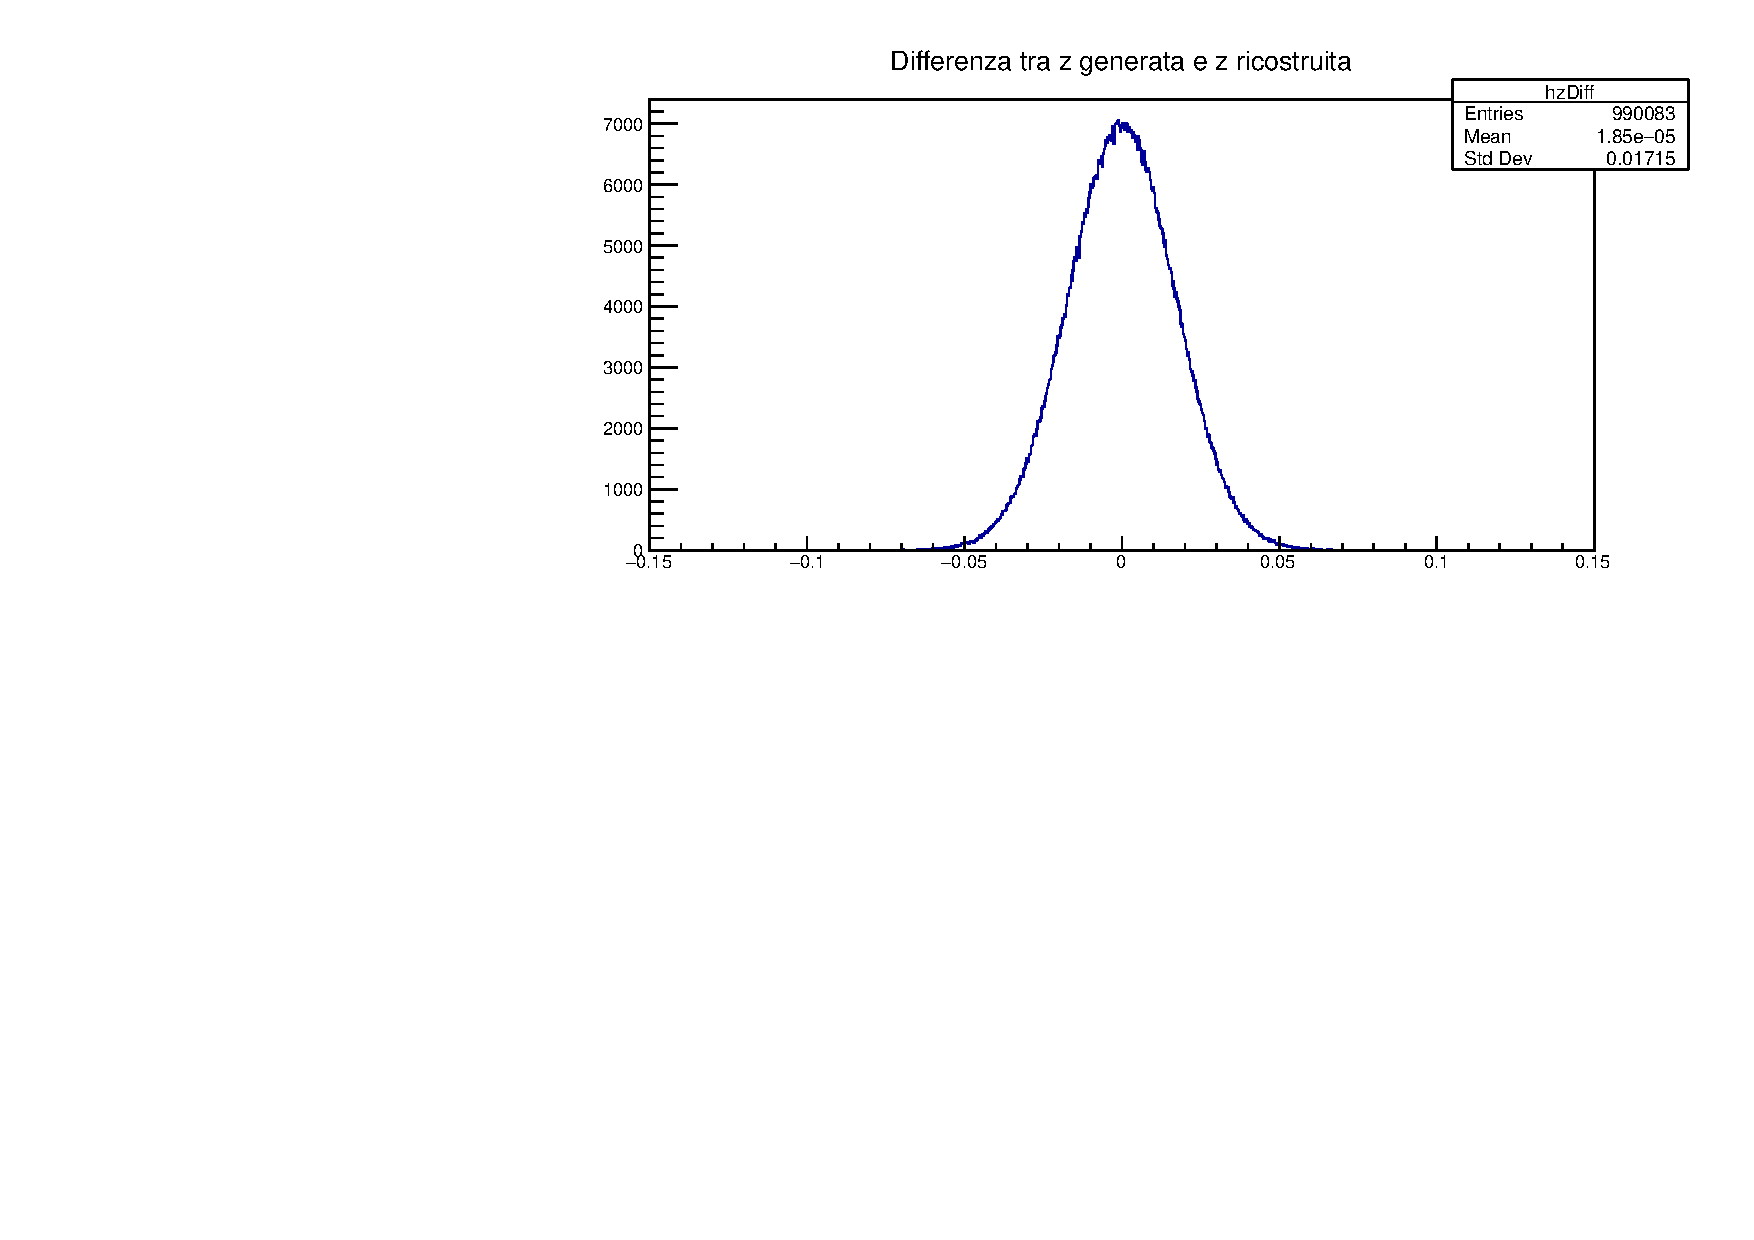
\includegraphics[width=0.47\textwidth]{Immagini/zDiff.pdf}
    \vspace{-5pt}
    \caption{Distribuzione degli scarti sulla variabile z}
    \label{zDIff}
    \vspace{-10pt}
\end{figure}
\par \noindent Come spiegato precedentemente, per valutare la coordinata $z$ del vertice ricostruito per ogni evento, è stato costruito un istogramma con tutti i possibili vertici dell'evento. Viene poi valutata la moda della distribuzione e presa come coordinata del vertice. La \figurename~\ref{istoModaBellissimo} e \figurename~\ref{istoModaBello} sono due esempi di distribuzione in cui la moda è ben definita. Nel primo caso tutti i possibili vertici sono raggruppati attorno al valore medio; nel secondo le possibili coppie di punti ricostruiscono il vertice sia attorno al picco, sia in posizioni più distanti.
\begin{figure}[h!]
   \vspace{-5pt}
  \centering
  \mbox{
   \begin{minipage}[1]{.47\textwidth}
     \centering
     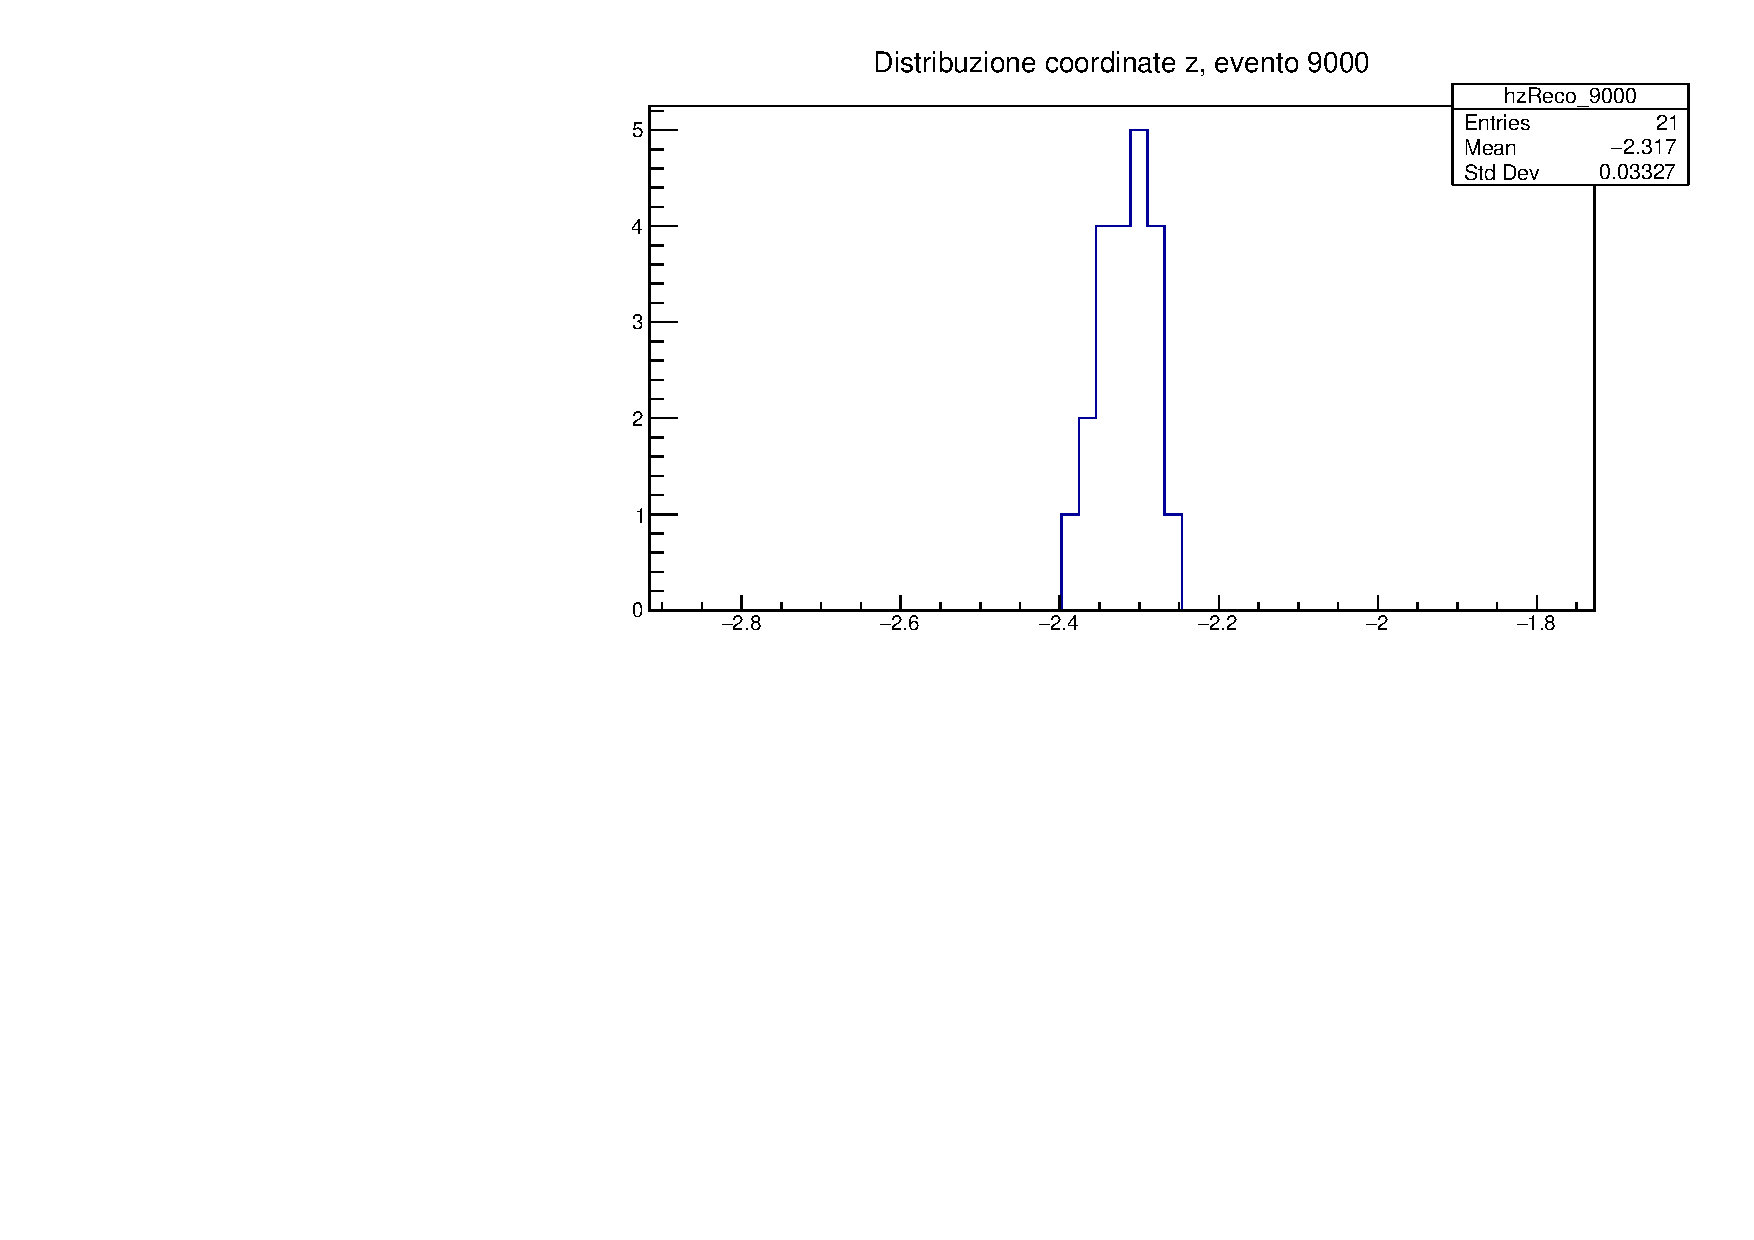
\includegraphics[width=0.95\textwidth]{Immagini/hzReco_picco_9000.pdf}
     \vspace{-5pt}
     \caption{Istogramma per valutare la moda della distribuzione dei vertici ricostruiti}
  \label{istoModaBellissimo}
   \end{minipage}
   \hspace{5mm}
   \begin{minipage}[r]{.47\textwidth}
     \centering
     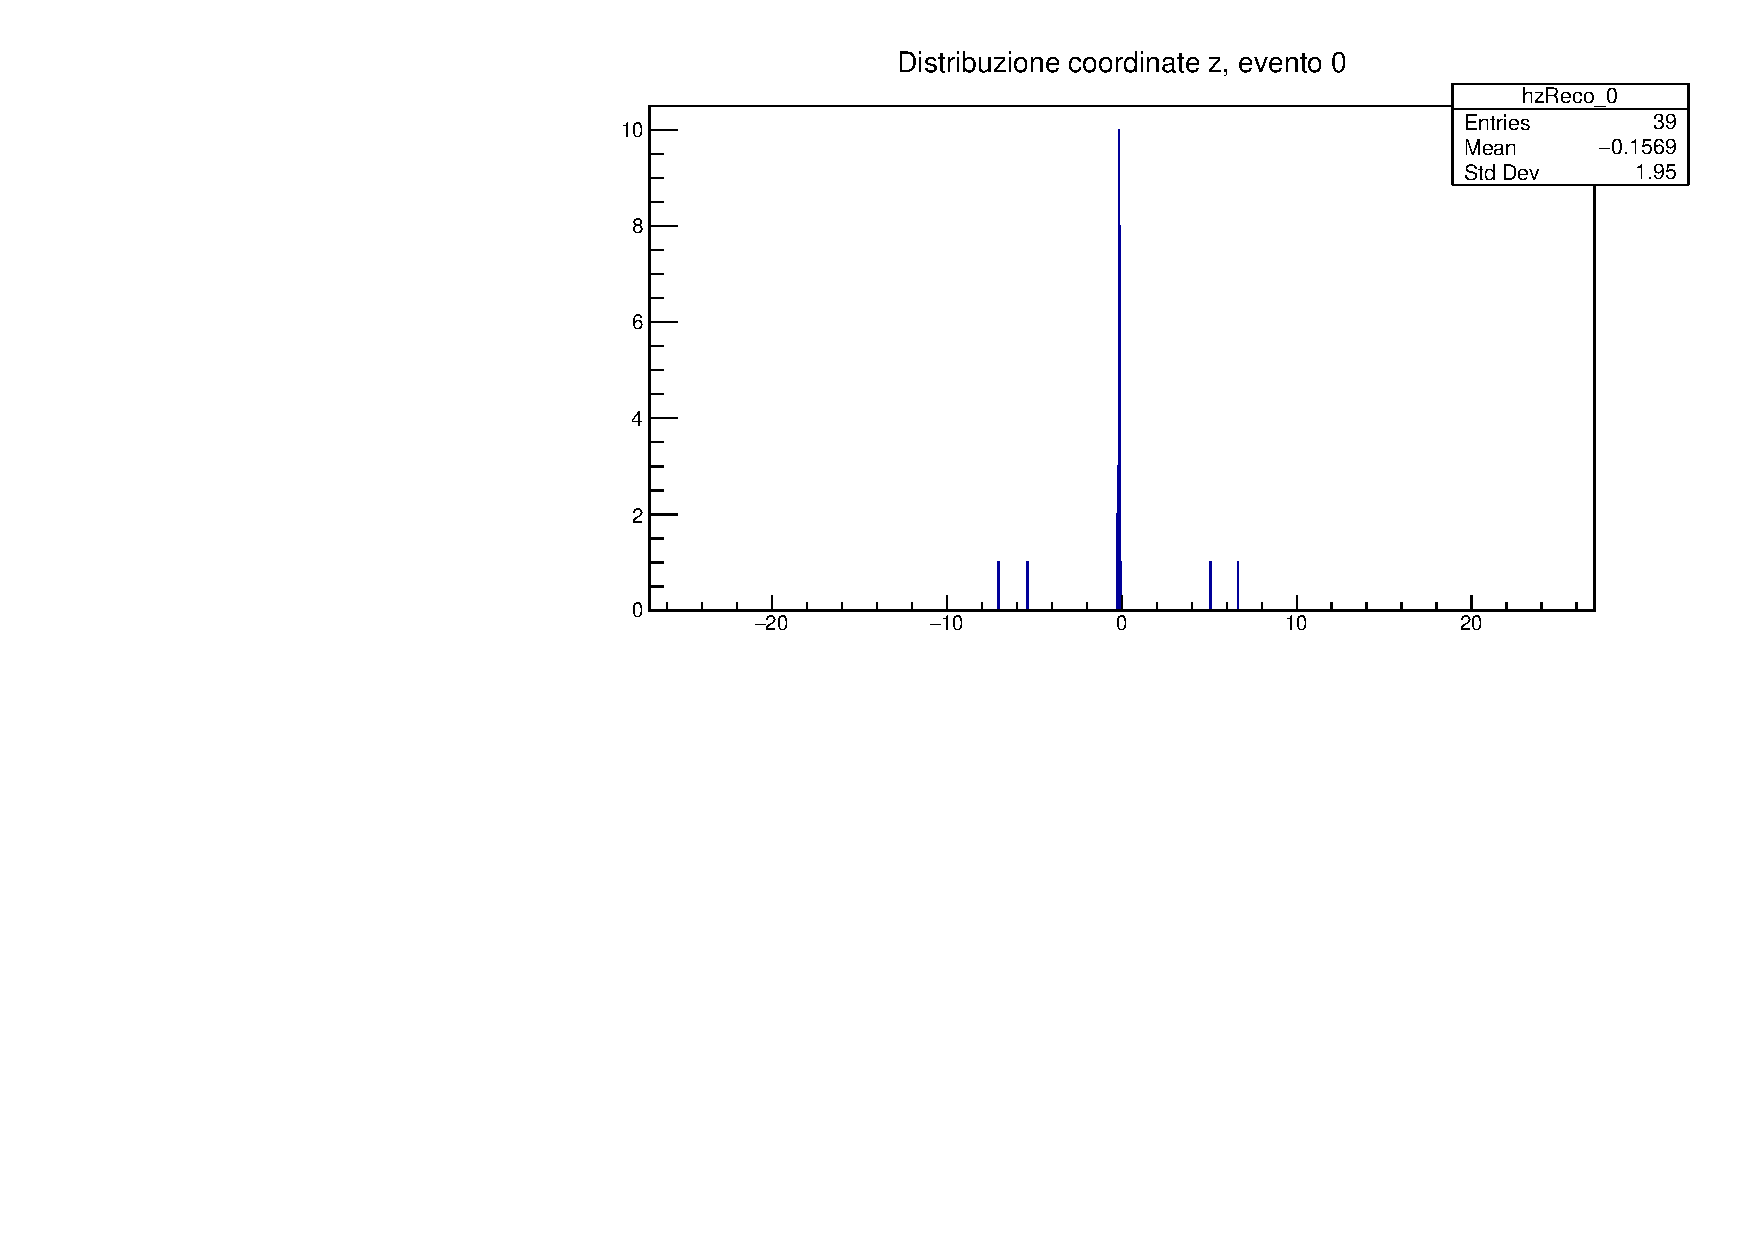
\includegraphics[width=0.95\textwidth]{Immagini/hzReco_bello_0.pdf}
     \vspace{-5pt}
     \caption{Istogramma per valutare la moda della distribuzione dei vertici ricostruiti}
  \label{istoModaBello}
   \end{minipage}}
   \vspace{-10pt}
\end{figure}

\begin{figure}[b]
    \centering
    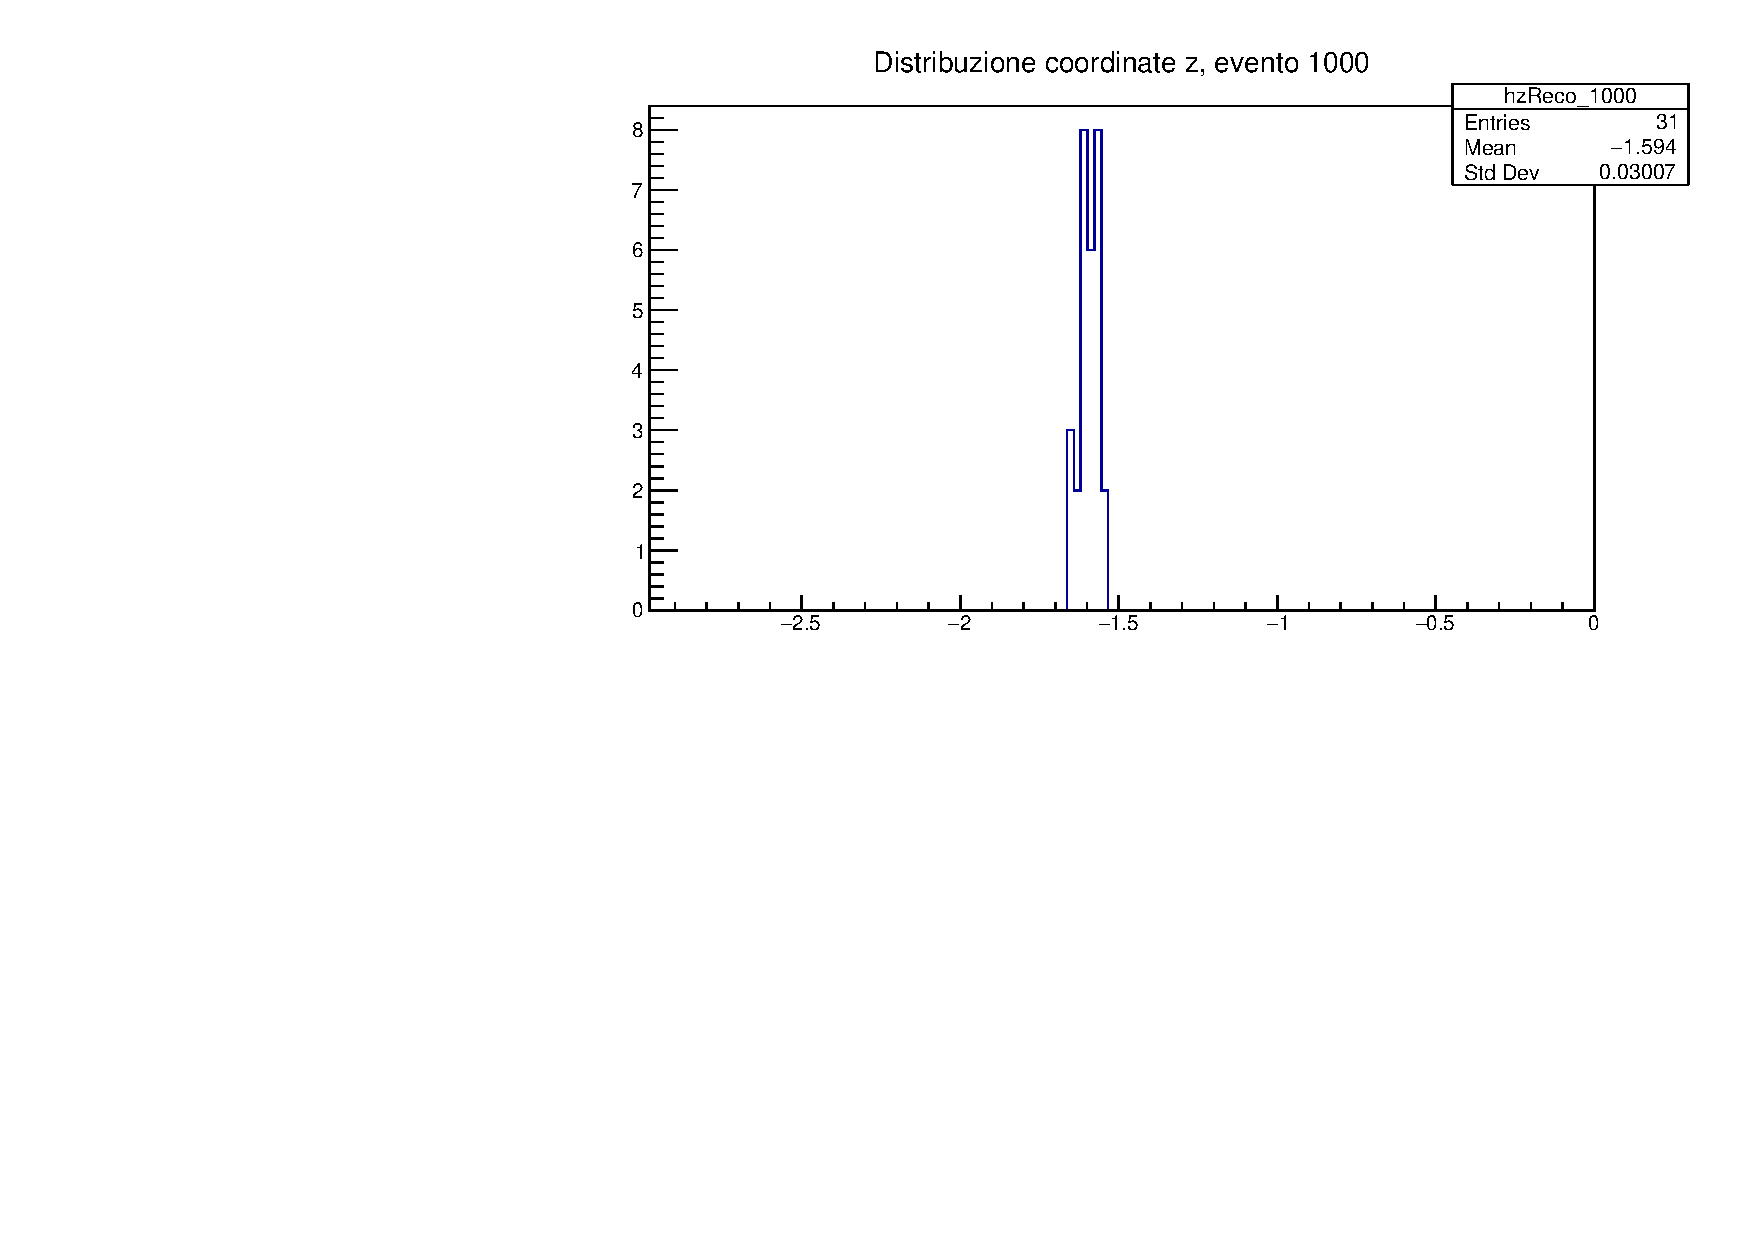
\includegraphics[width=0.47\textwidth]{Immagini/hzReco_medio_1000.pdf}
    \vspace{-5pt}
    \caption{Istogramma per valutare la moda della distribuzione dei vertici ricostruiti}
    \label{istoModaMedio}
    \vspace{-10pt}
\end{figure}
\noindent Invece, in \figurename~\ref{istoModaMedio} si può vedere che la distribuzione è bimodale. In questo caso la funzione \lstinline{Moda} effettua una media dei due massimi se essi sono sufficientemente vicini, altrimenti prende il valore del massimo più vicino a $z = 0$.

\noindent Alcune ricostruzioni però possono non dare risultati. In \figurename~\ref{istoModaBrutto} viene riportato il caso in cui non è presente una moda della distribuzione, perché tutte le possibili coppie portano a ricostruire un vertice diverso. In questo caso, il vertice non viene ricostruito.\\
In \figurename~\ref{istoModaVuoto} viene riportato un grafico vuoto: questo è dovuto al fatto che nessuna delle coppie possibili riesce a ricostruire un possibile vertice.

\begin{figure}[h!]
  \vspace{-5pt}
  \centering
  \mbox{
   \begin{minipage}[1]{.47\textwidth}
     \centering
     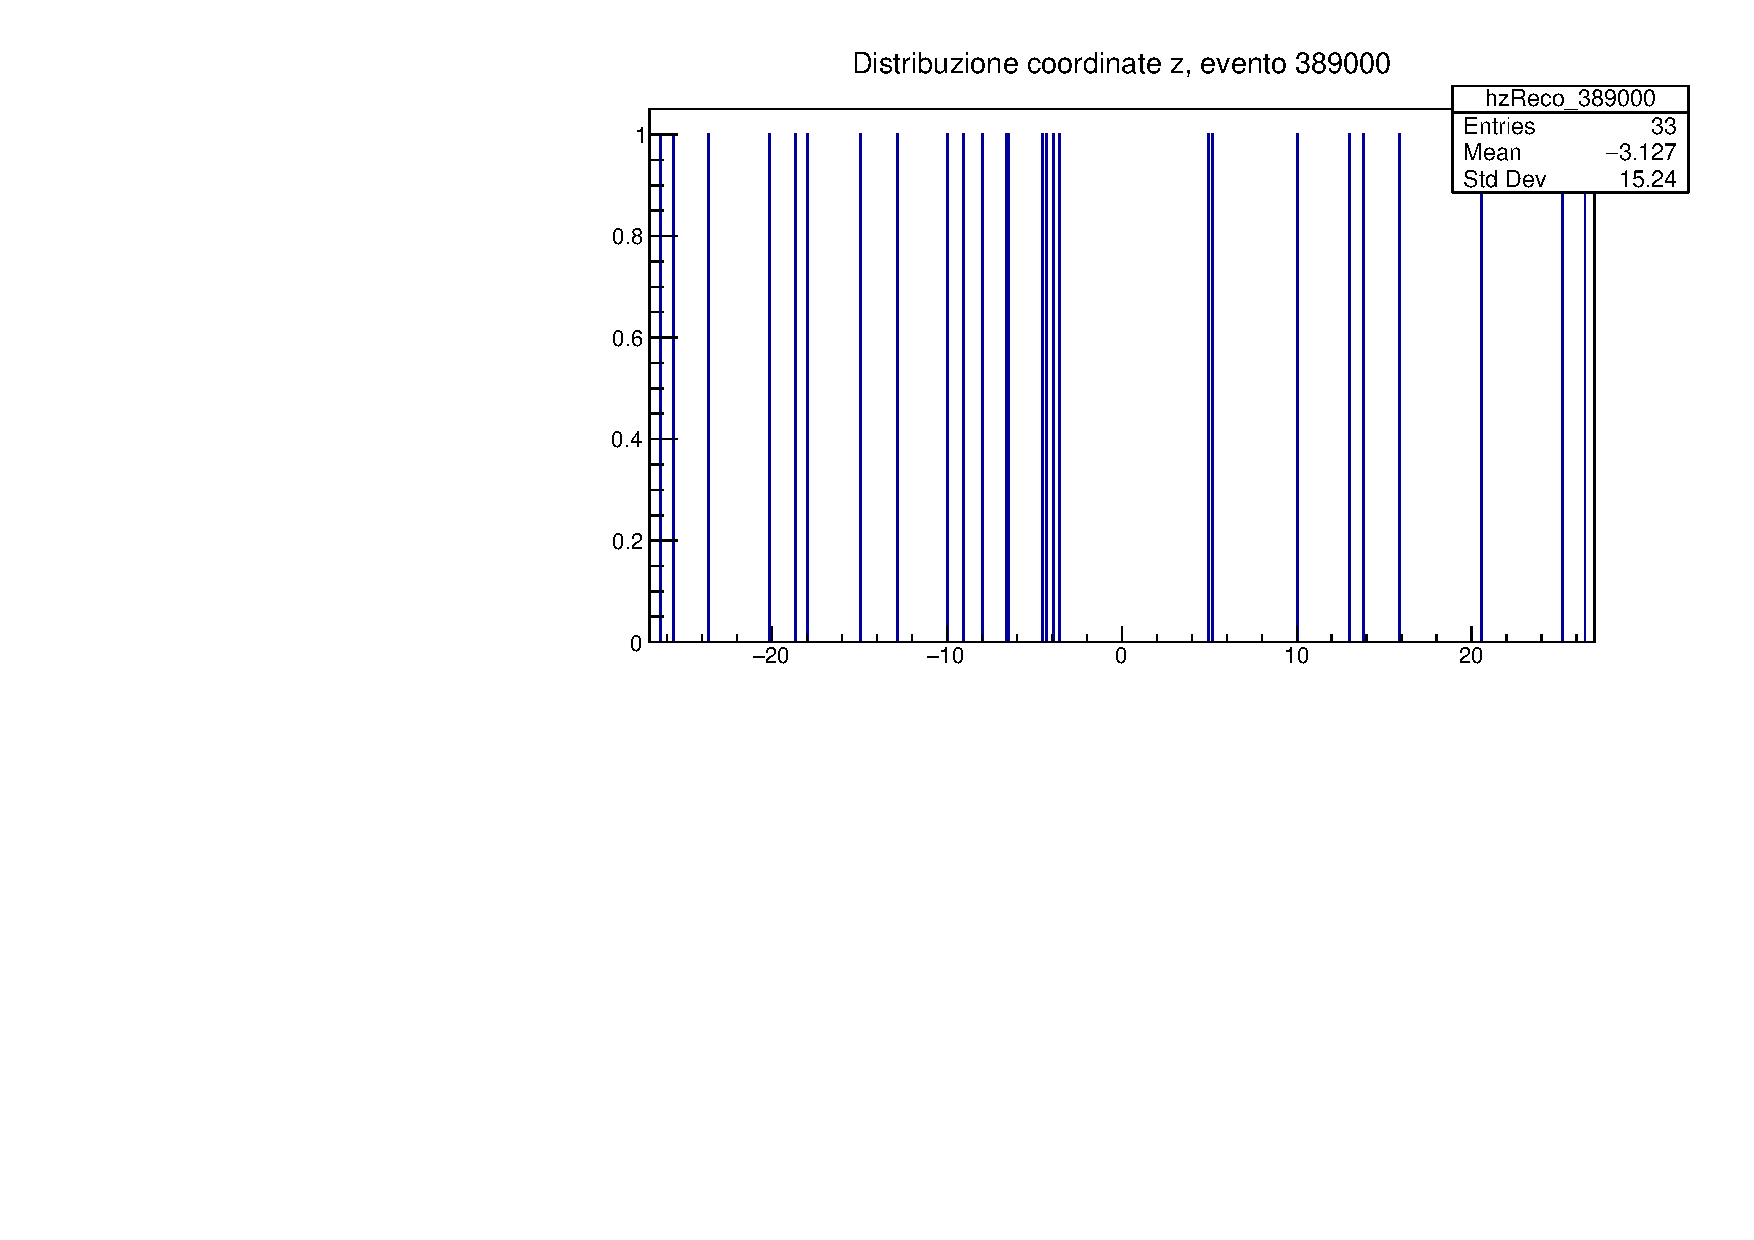
\includegraphics[width=0.95\textwidth]{Immagini/hzReco_389k.pdf}
     \vspace{-5pt}
     \caption{Istogramma per valutare la moda della distribuzione dei vertici ricostruiti}
  \label{istoModaBrutto}
   \end{minipage}
   \hspace{5mm}
   \begin{minipage}[r]{.47\textwidth}
     \centering
     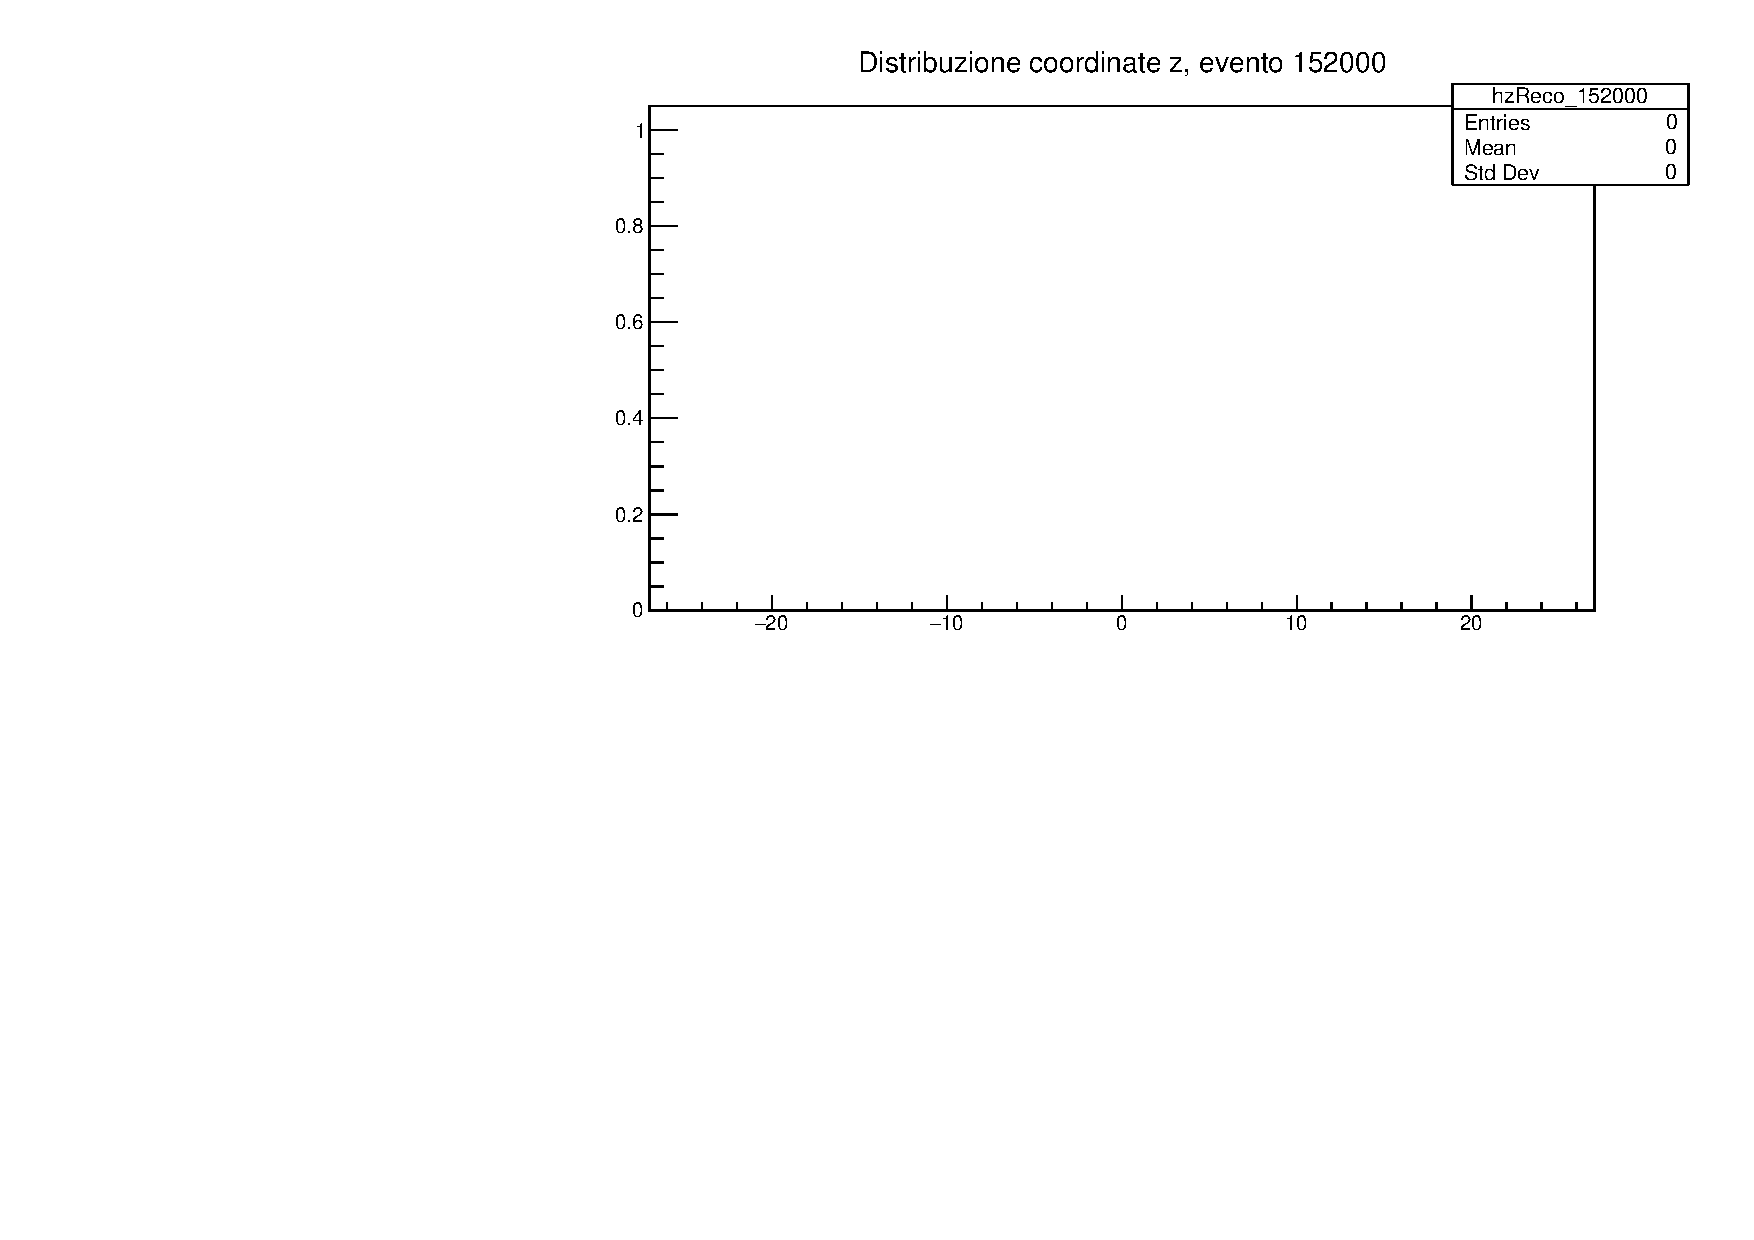
\includegraphics[width=0.95\textwidth]{Immagini/hzReco_vuoto_152k.pdf}
     \vspace{-5pt}
     \caption{Istogramma per valutare la moda della distribuzione dei vertici ricostruiti}
  \label{istoModaVuoto}
   \end{minipage}}
    \vspace{-10pt}
\end{figure}

Infine vengono proposti alcuni confronti di ricostruzione in presenza di diverse magnitudini di rumore. Sono state effettuate quattro ricostruzioni e analisi con livelli di rumore crescente: 0, 10, 50 o 100 punti di rumore per ogni layer. In \figurename~\ref{RumoreRisz} viene riportato il confronto della risoluzione dell'apparato in funzione della posizione del vertice dell'evento, mentre in \figurename~\ref{RumoreRismolt} si può osservare come varia la risoluzione dell'apparato in funzione della molteplicità, entrambi all'aumentare del rumore sui due layer.

\begin{figure}[h!]
  \vspace{-5pt}
  \centering
  \mbox{
   \begin{minipage}[1]{.47\textwidth}
     \centering
     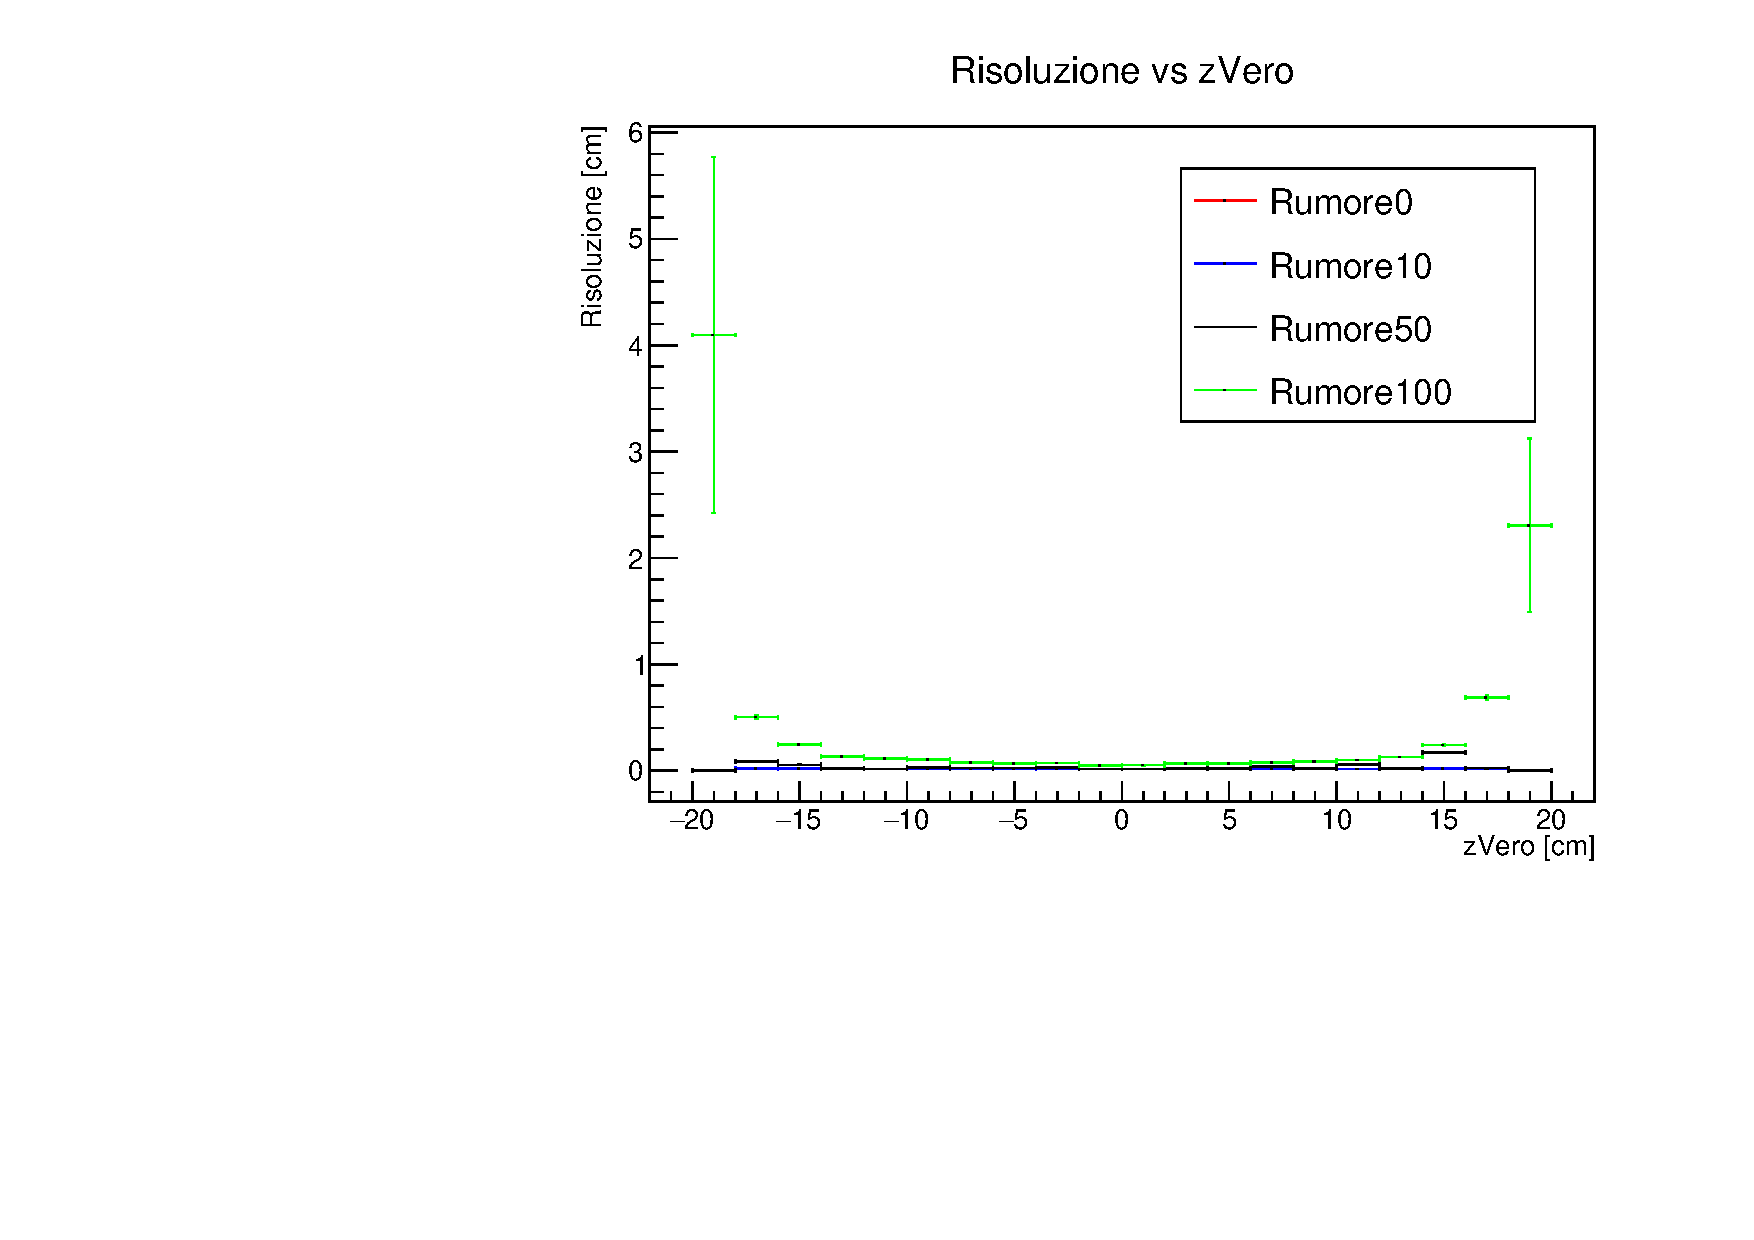
\includegraphics[width=0.95\textwidth]{Immagini/risoluzione_1_tutte.pdf}
  \vspace{-5pt}
     \caption{Confronto della risoluzione dell'apparato in funzione della posizione del vertice}
  \label{RumoreRisz}
   \end{minipage}
   \hspace{5mm}
   \begin{minipage}[r]{.47\textwidth}
     \centering
     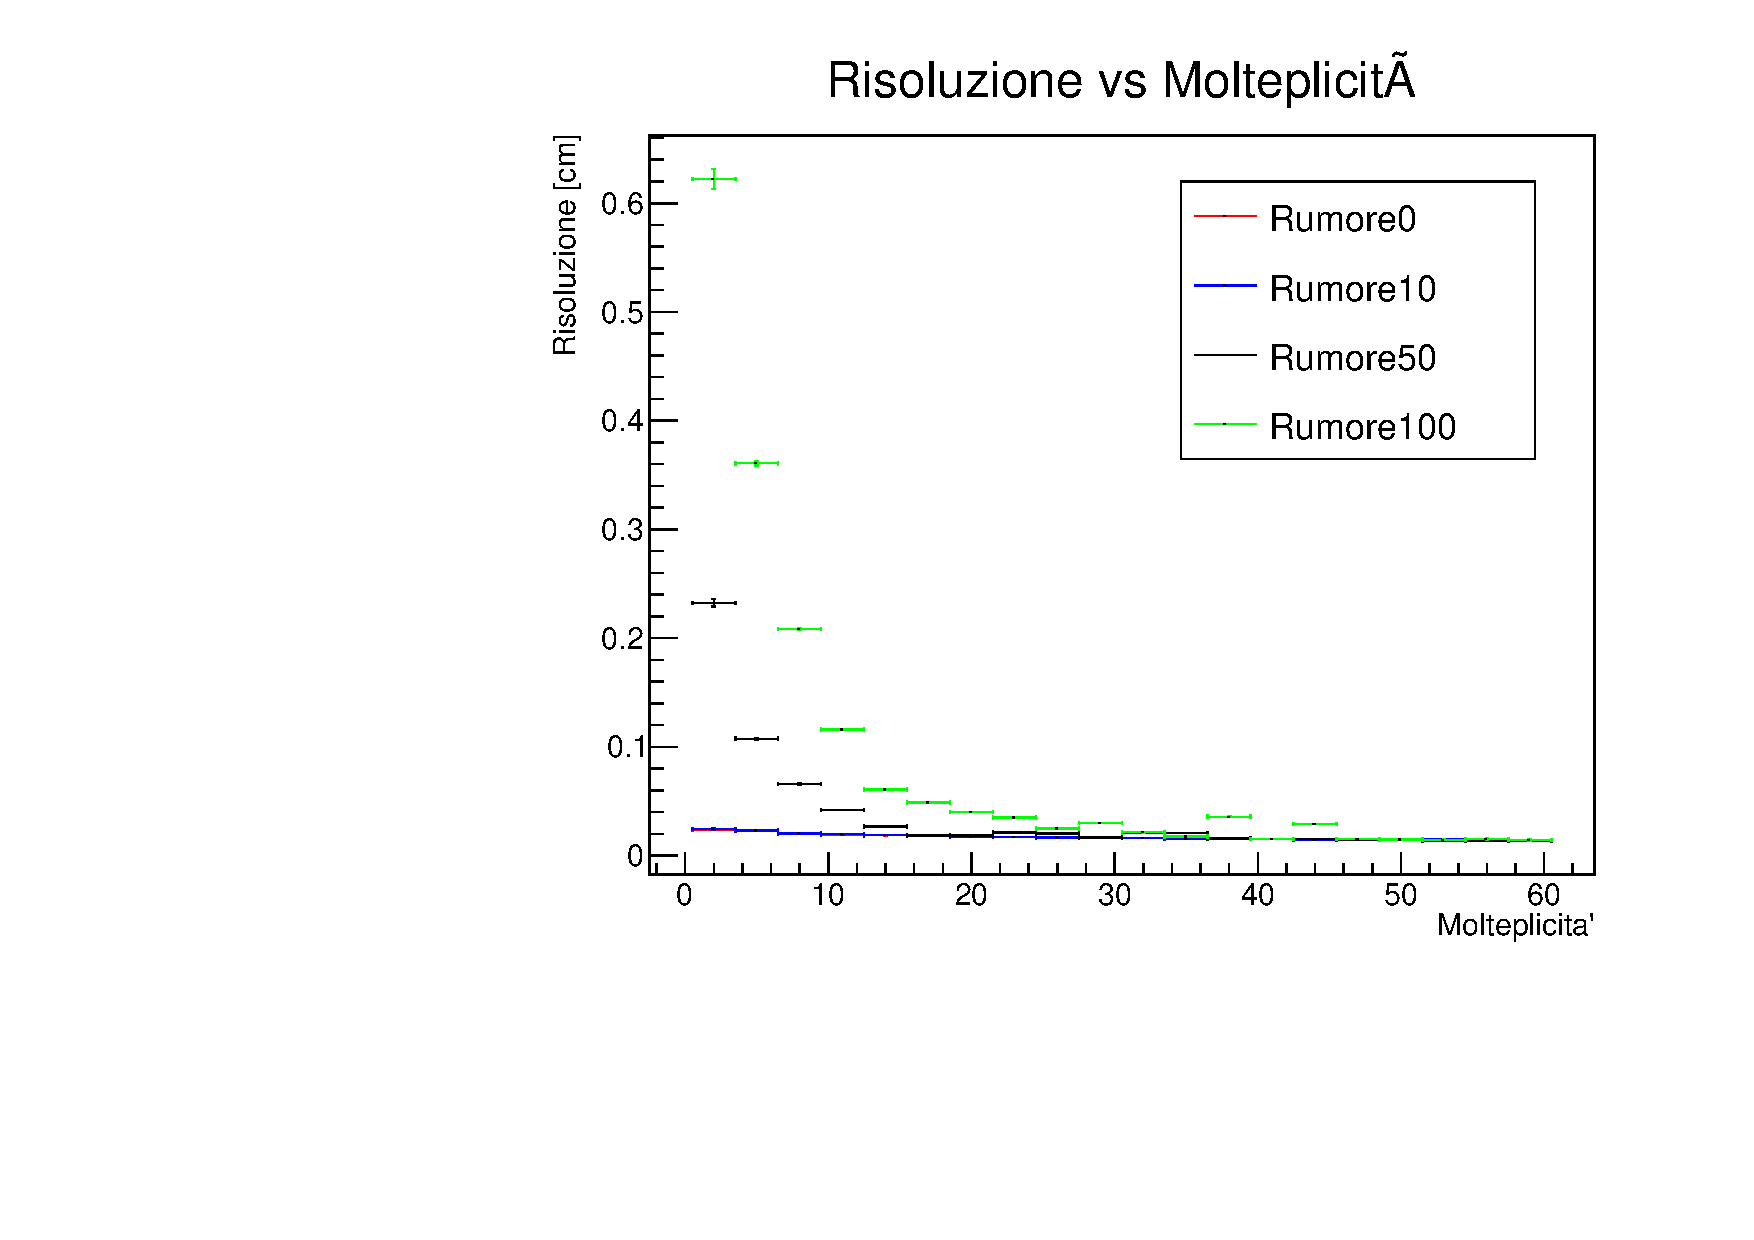
\includegraphics[width=0.95\textwidth]{Immagini/risoluzione_0_tutte.pdf}
  \vspace{-5pt}
     \caption{Confronto della risoluzione dell'apparato in funzione della molteplicità}
  \label{RumoreRismolt}
   \end{minipage}}
  \vspace{-10pt}
\end{figure}

\par \noindent In \figurename~\ref{RumoreRiszno100} e \figurename~\ref{RumoreRismoltno100} vengono riportati anche i grafici di confronto in assenza dell'analisi con 100 punti di rumore per layer, per poter osservare meglio le curve che altrimenti vengono schiacciate verso l'asse delle ascisse a causa della curva a rumore maggiore.

\begin{figure}[h!]
  \centering
  \vspace{-5pt}
  \mbox{
   \begin{minipage}[1]{.48\textwidth}
     \centering
     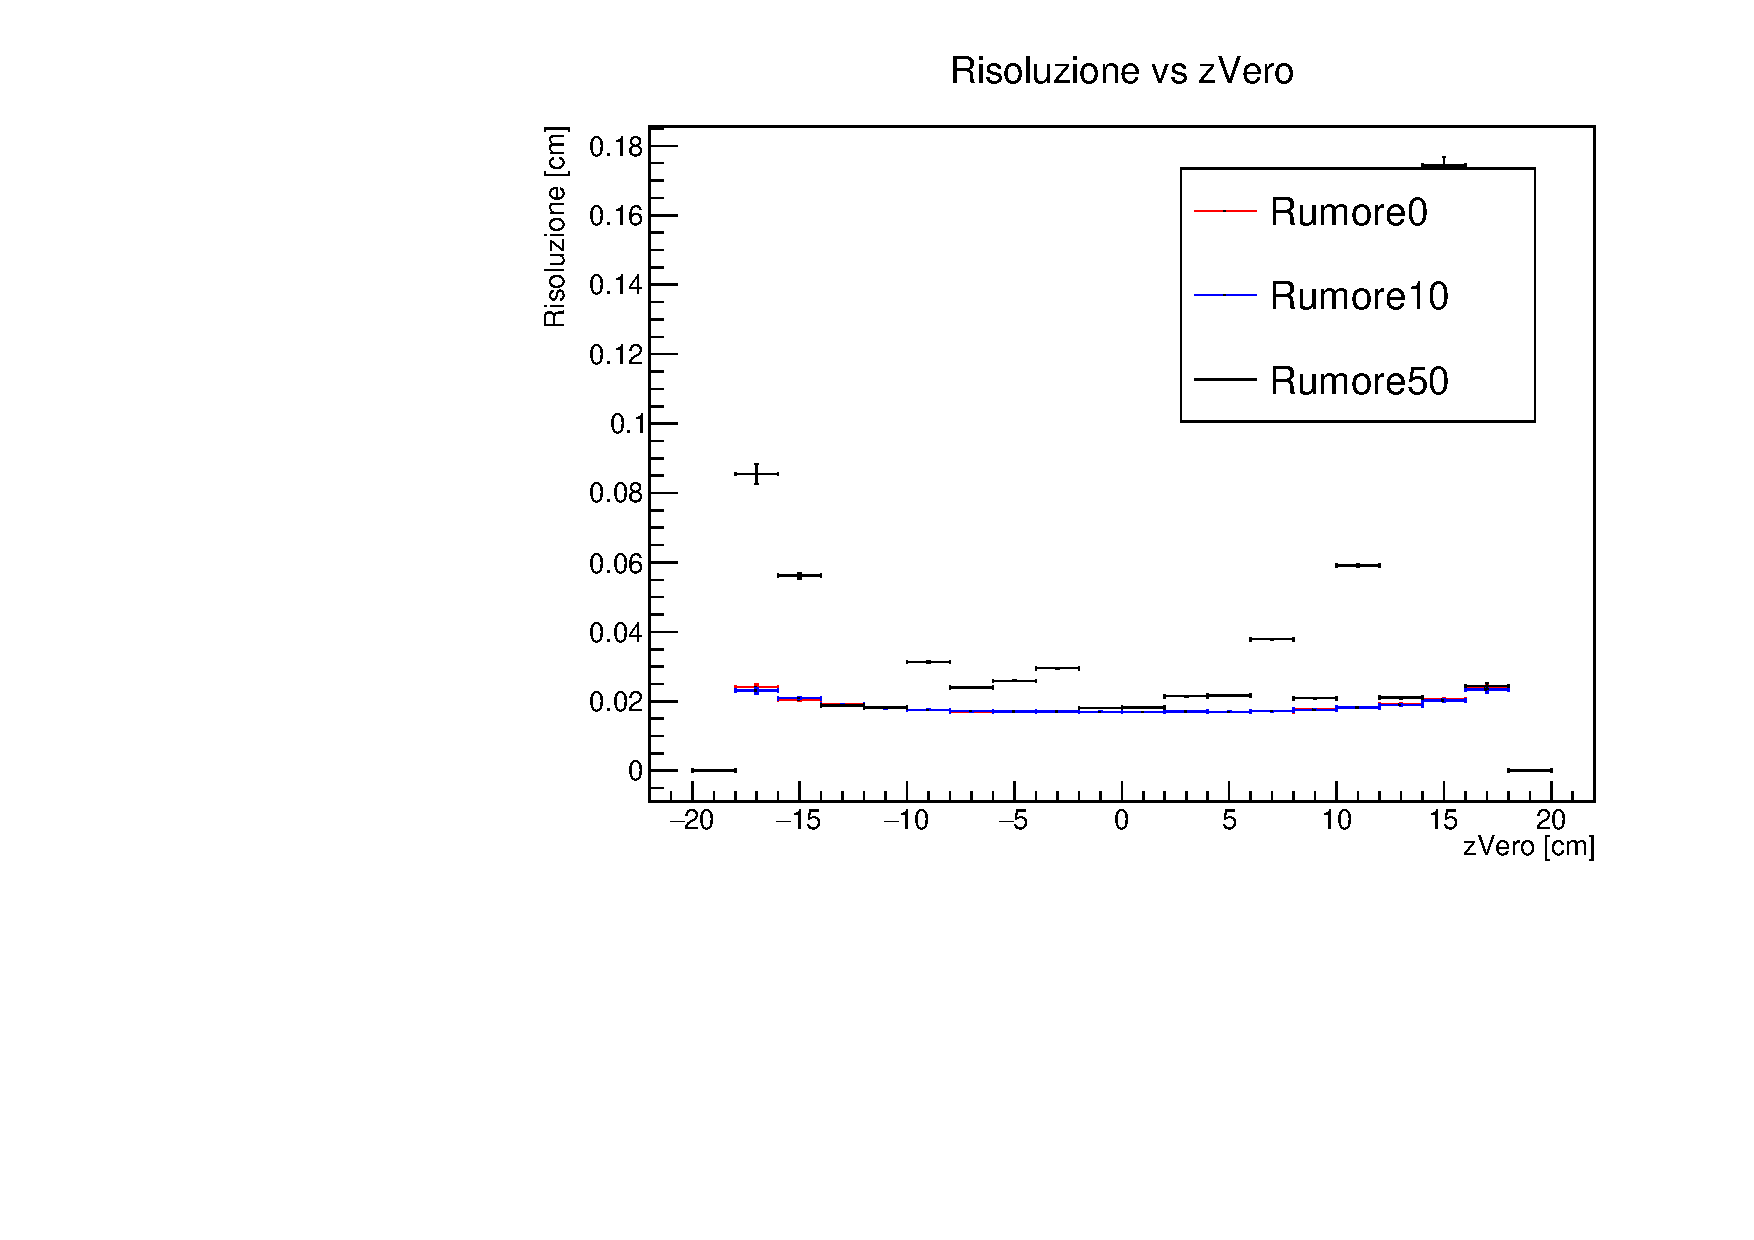
\includegraphics[width=0.95\textwidth]{Immagini/risoluzione_1_no_rumore100.pdf}
  \vspace{-5pt}
     \caption{Confronto della risoluzione dell'apparato in funzione della posizione del vertice escludendo la curva per 100 punti di rumore per layer}
  \label{RumoreRiszno100}
   \end{minipage}
   \hspace{3mm}
   \begin{minipage}[r]{.48\textwidth}
     \centering
     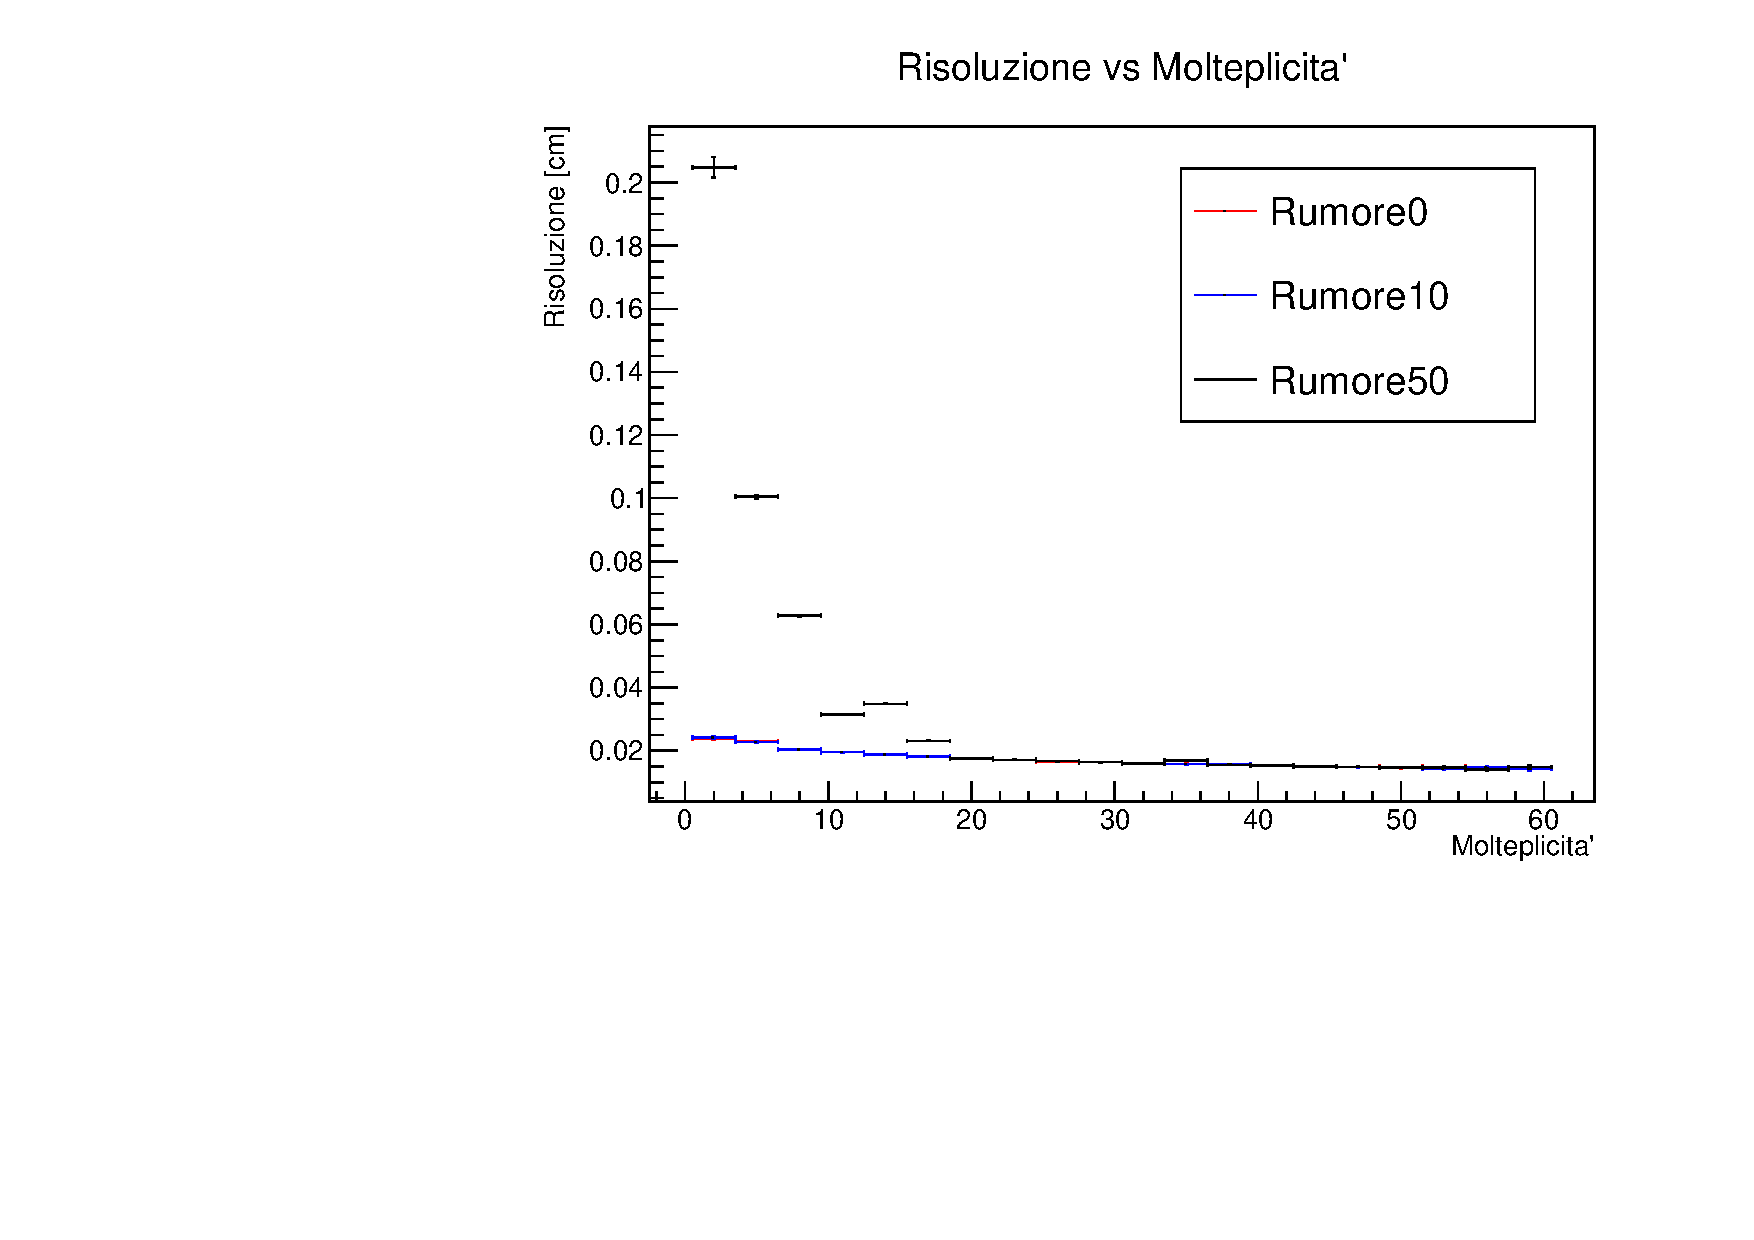
\includegraphics[width=0.95\textwidth]{Immagini/risoluzione_0_no_rumore100.pdf}
  \vspace{-5pt}
     \caption{Confronto della risoluzione dell'apparato in funzione della molteplicità escludendo la curva per 100 punti di rumore per layer}
  \label{RumoreRismoltno100}
   \end{minipage}}
  \vspace{-20pt}
\end{figure}

\newpage
\par Analogamente, vengono riportati anche i confronti al variare del rumore per l'efficienza di ricostruzione dell'apparato in funzione della molteplicità dell'evento. In \figurename~\ref{effMoltTutti} viene valutata l'efficienza di ricostruzione su tutti gli eventi della simulazione, mentre in \figurename~\ref{effMoltTuttino100} il confronto escludendo la ricostruzione con 100 punti di rumore. In \figurename~\ref{effMolt1s} e \figurename~\ref{effMolt1sno100} si valuta l'efficienza selezionando solo gli eventi che hanno una generazione del vertice entro $1\sigma$ da $z=0$ e in \figurename~\ref{effMolt3s} e \figurename~\ref{effMolt3sno100} l'efficienza selezionando gli eventi entro $3\sigma$ da $z=0$.

\begin{figure}[h!]
  \centering
  \mbox{
   \begin{minipage}[1]{.47\textwidth}
     \centering
     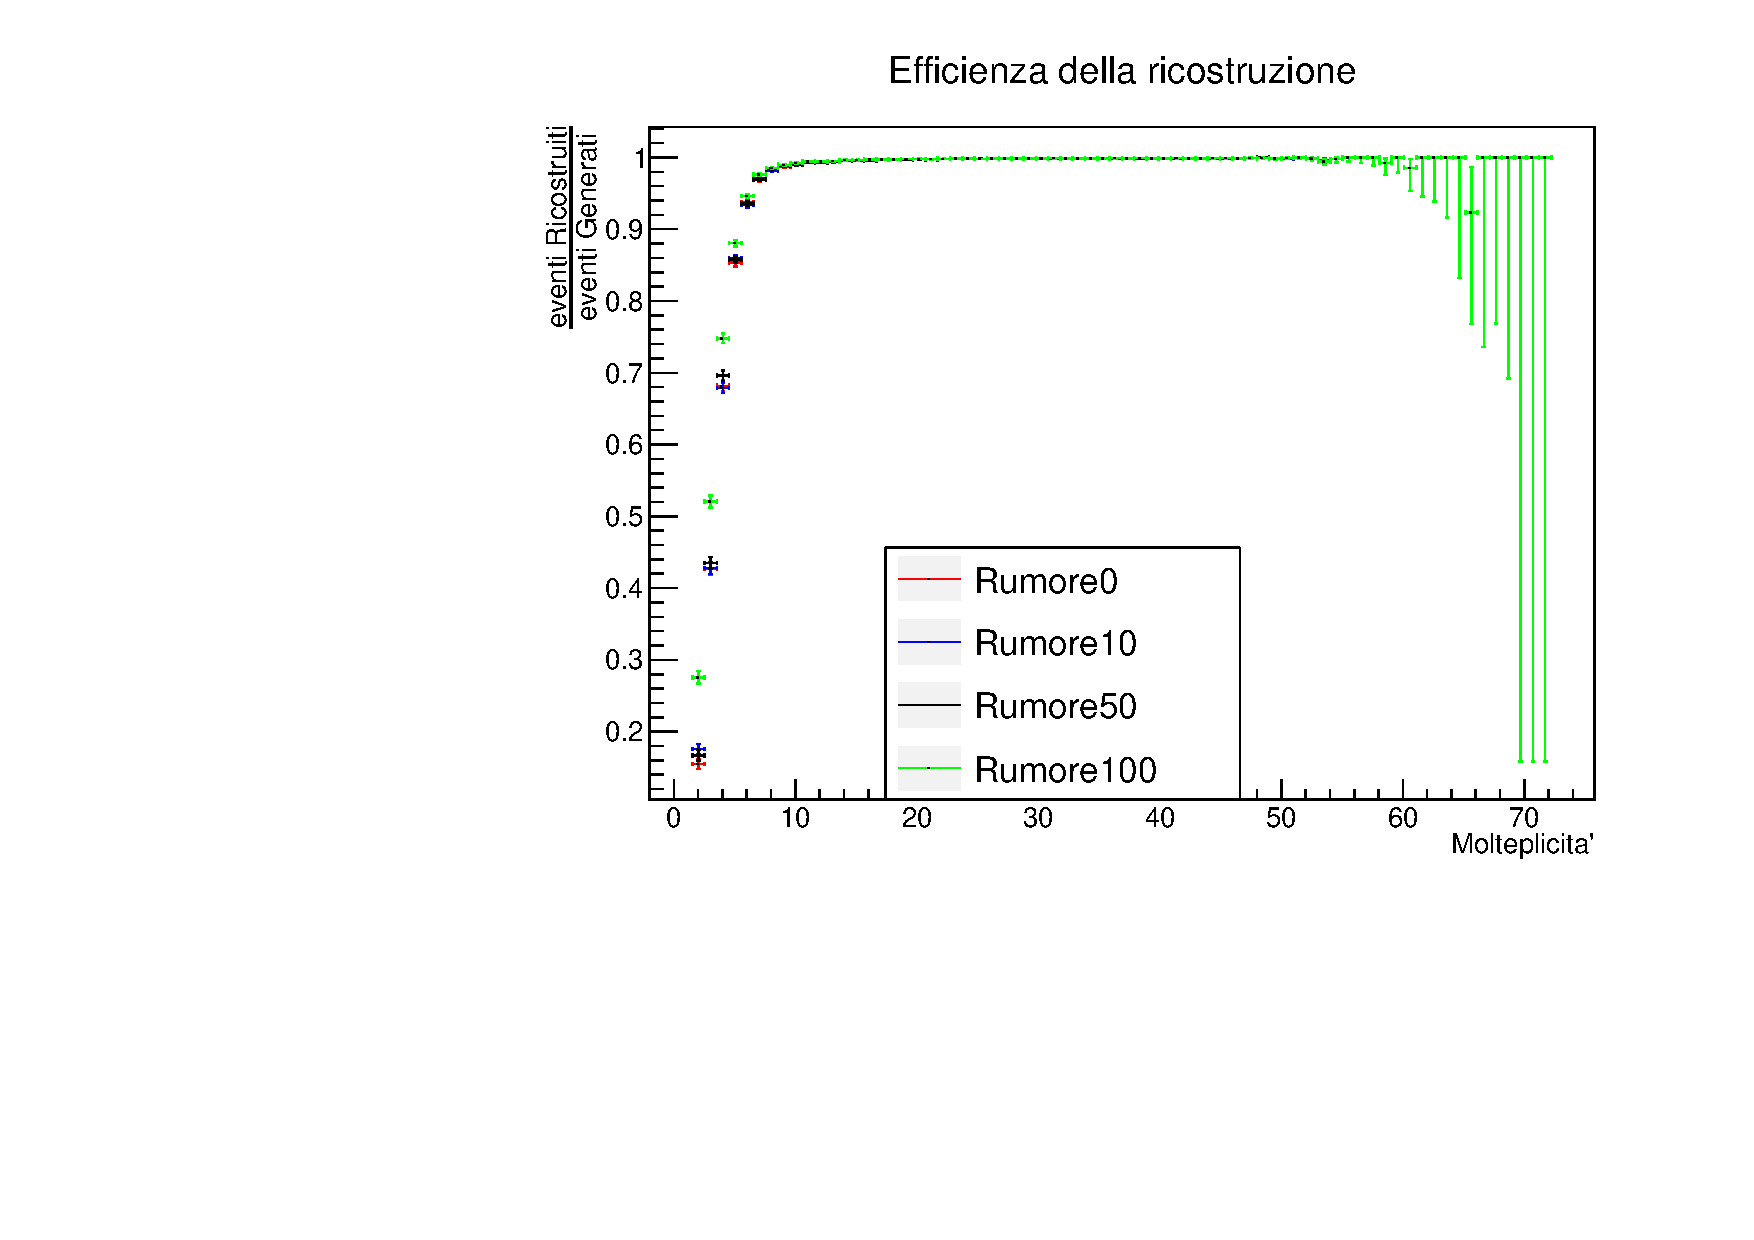
\includegraphics[width=0.95\textwidth]{Immagini/efficienza_molteplicita_0_tutte.pdf}
     %\vspace{-15pt}
     \caption{Efficienza di ricostruzione in funzione della molteplicità valutando tutti gli eventi}
  \label{effMoltTutti}
   \end{minipage}
   \hspace{5mm}
   \begin{minipage}[r]{.47\textwidth}
     \centering
     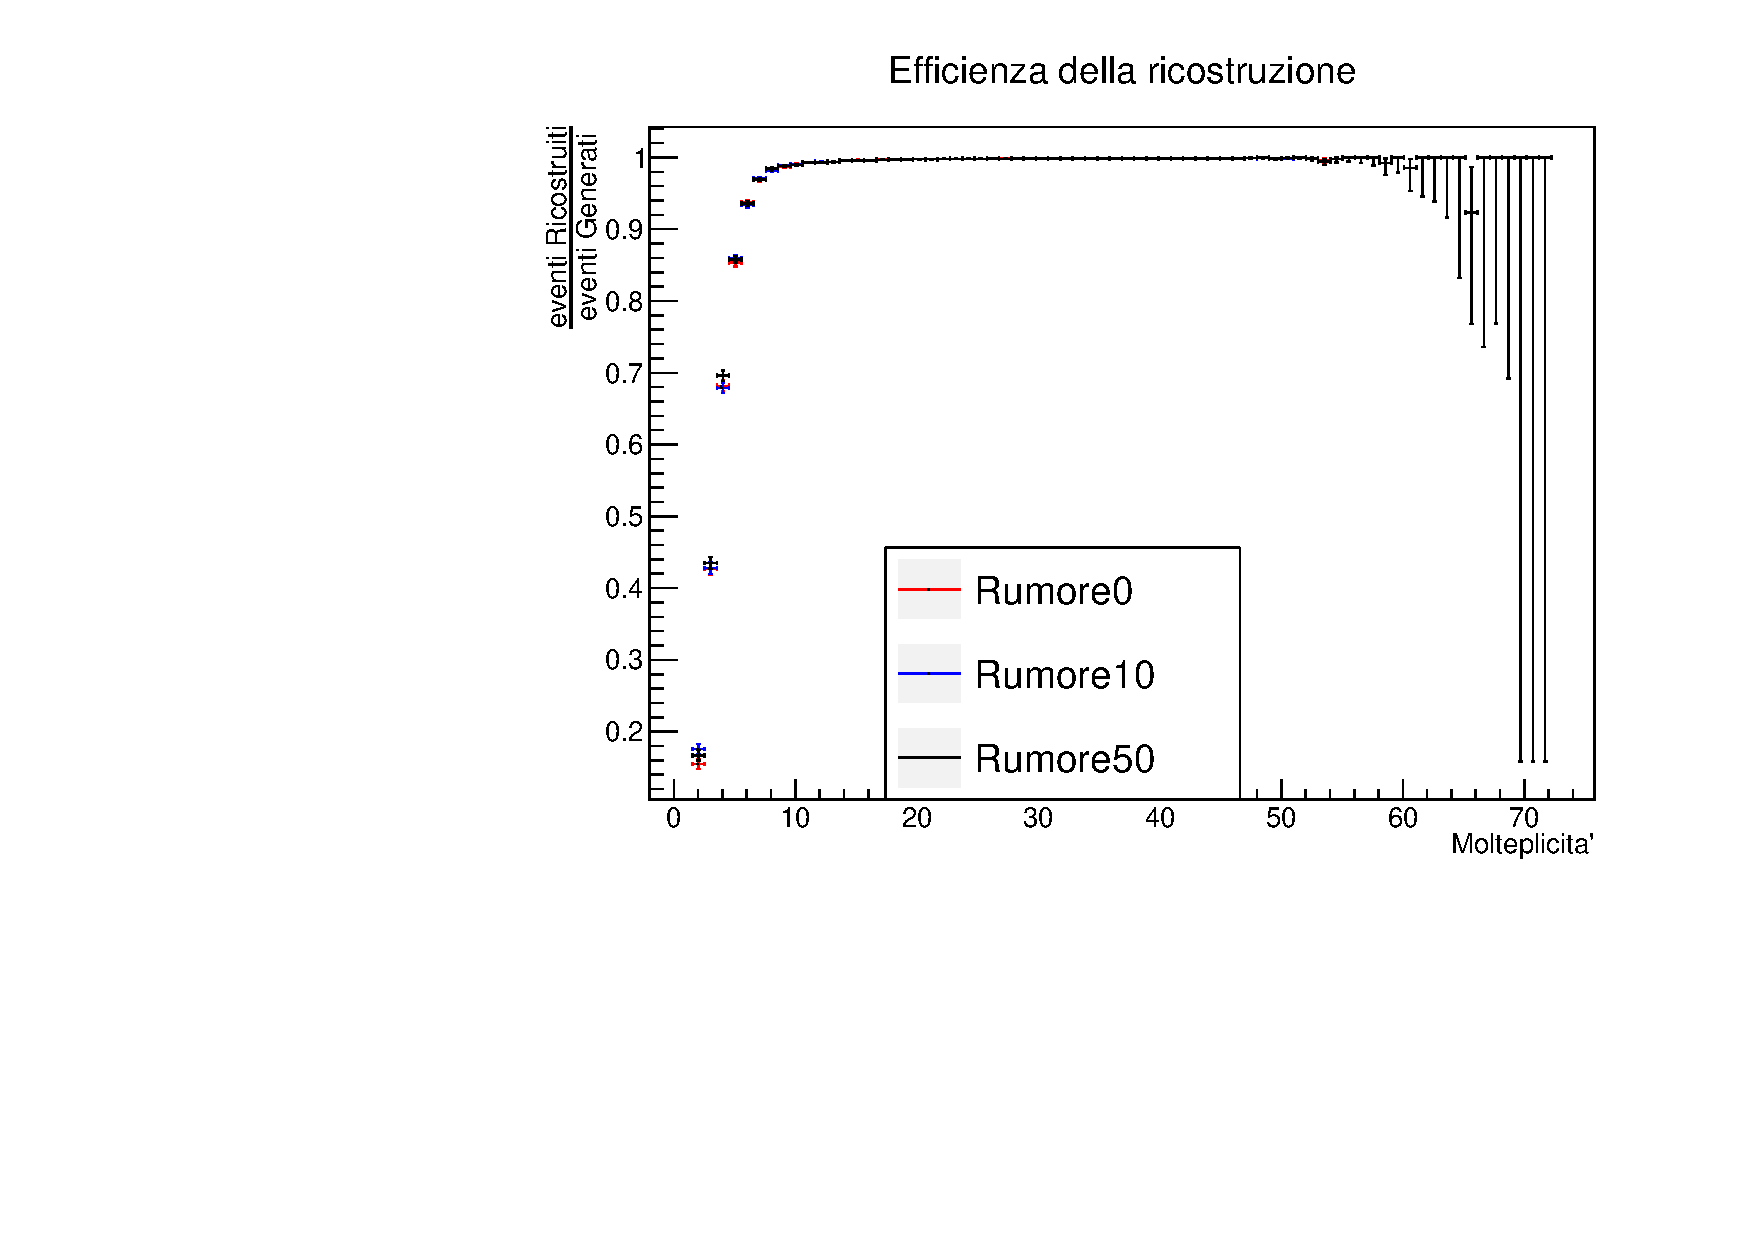
\includegraphics[width=0.95\textwidth]{Immagini/efficienza_molteplicita_0_no_rumore100.pdf}
     %\vspace{-15pt}
     \caption{Efficienza di ricostruzione in funzione della molteplicità valutando tutti gli eventi escludendo l'analisi con 100 punti di rumore}
  \label{effMoltTuttino100}
   \end{minipage}}
\end{figure}

\begin{figure}[h!]
  \centering
  \mbox{
   \begin{minipage}[1]{.47\textwidth}
     \centering
     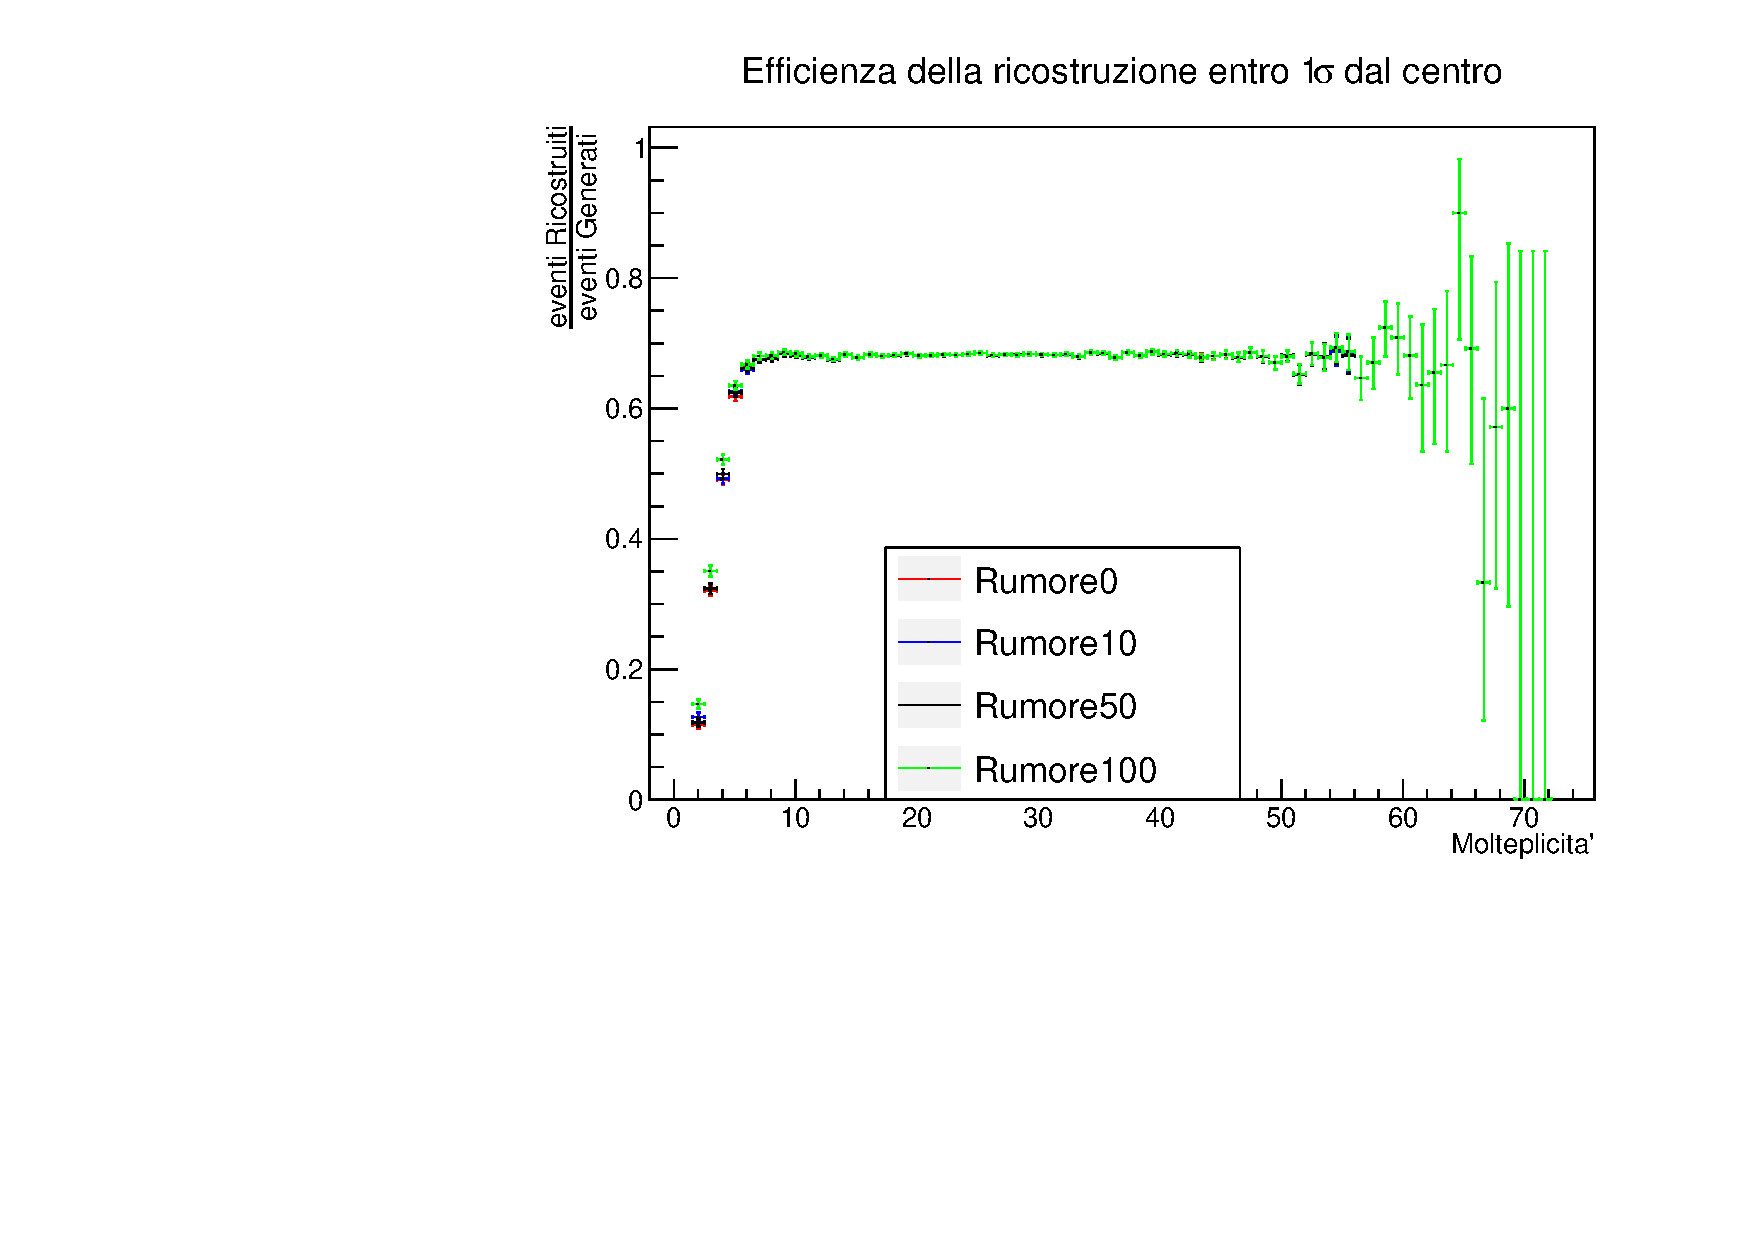
\includegraphics[width=0.95\textwidth]{Immagini/efficienza_molteplicita_1_tutte.pdf}
     %\vspace{-15pt}
     \caption{Efficienza di ricostruzione in funzione della molteplicità valutando gli eventi entro 1$\sigma$}
  \label{effMolt1s}
   \end{minipage}
   \hspace{5mm}
   \begin{minipage}[r]{.47\textwidth}
     \centering
     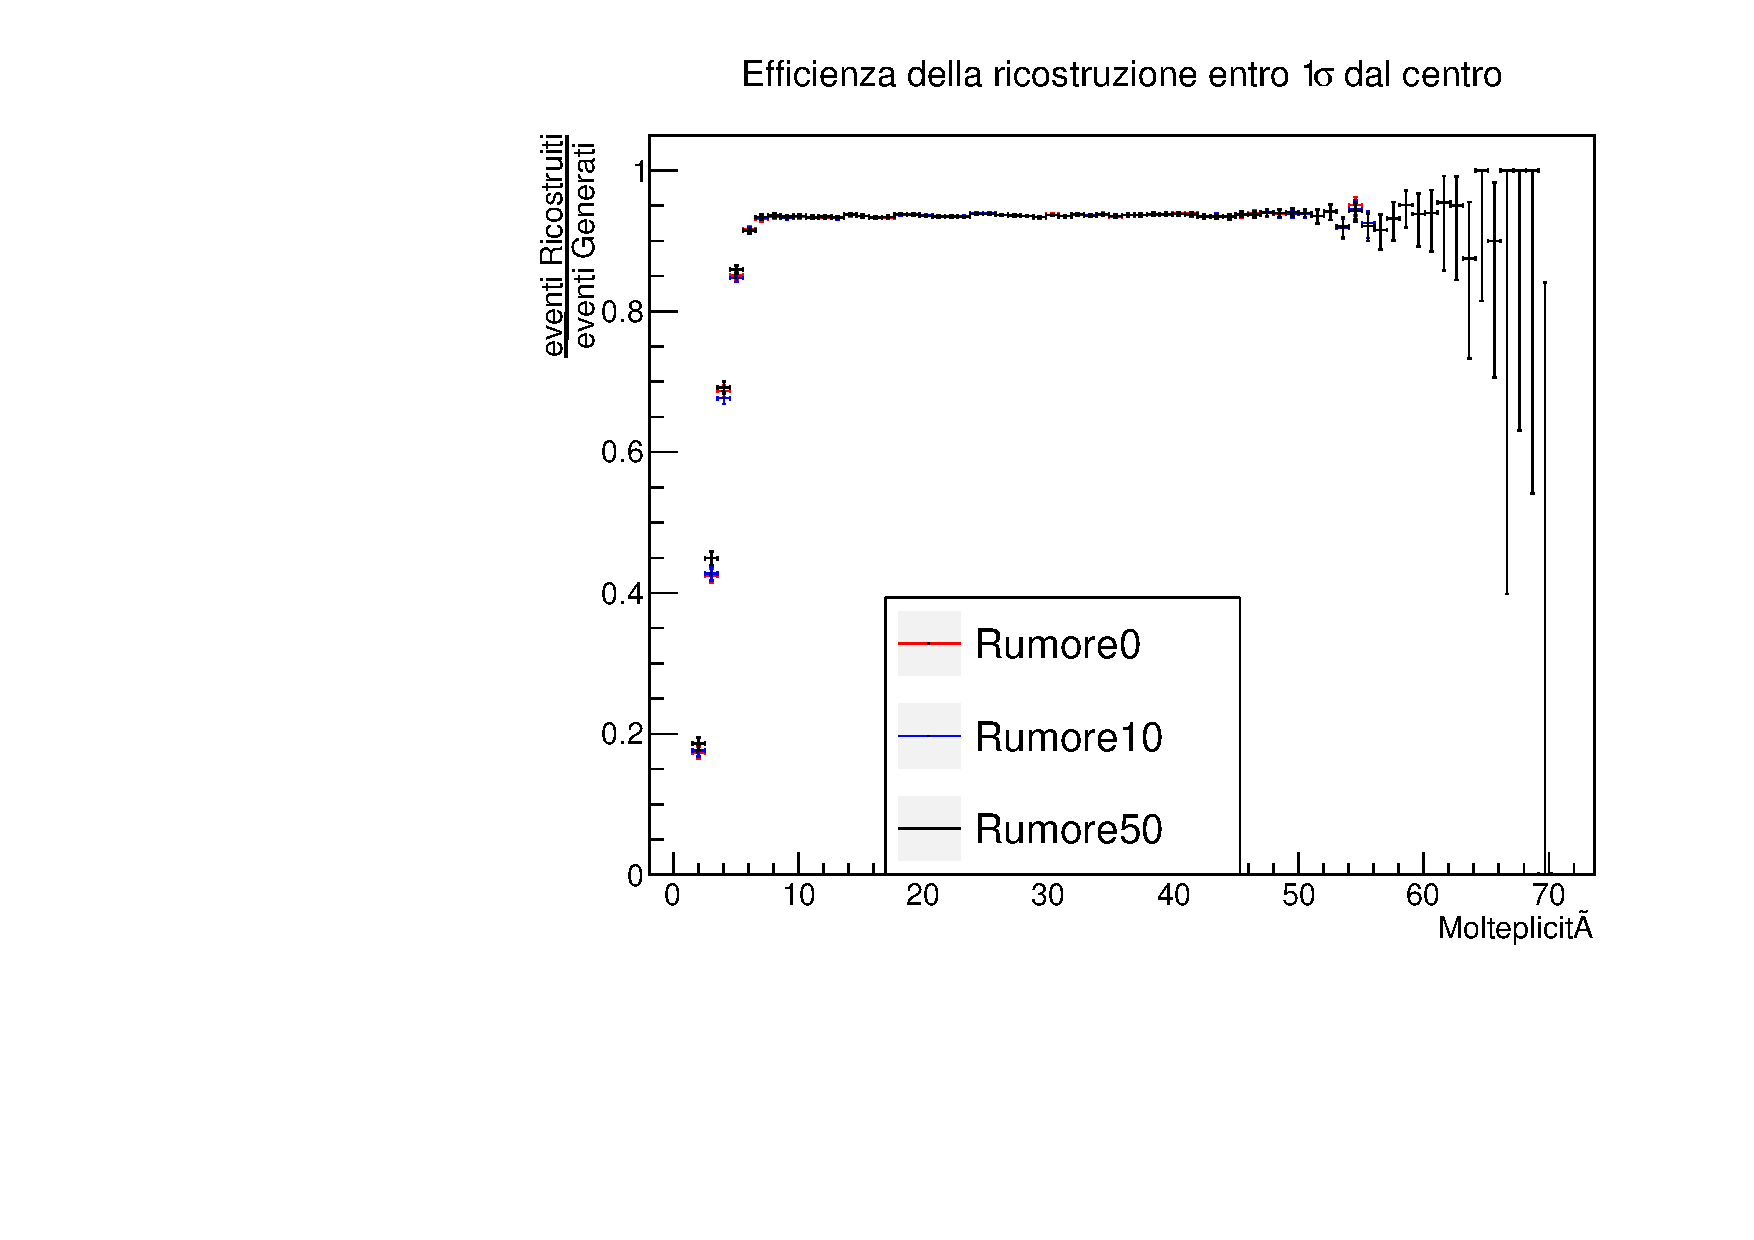
\includegraphics[width=0.95\textwidth]{Immagini/efficienza_molteplicita_1_no_rumore100.pdf}
     %\vspace{-15pt}
     \caption{Efficienza di ricostruzione in funzione della molteplicità valutando gli eventi entro 1$\sigma$ escludendo l'analisi con 100 punti di rumore}
  \label{effMolt1sno100}
   \end{minipage}}
\end{figure}

\begin{figure}[h!]
  \centering
  \mbox{
   \begin{minipage}[1]{.47\textwidth}
     \centering
     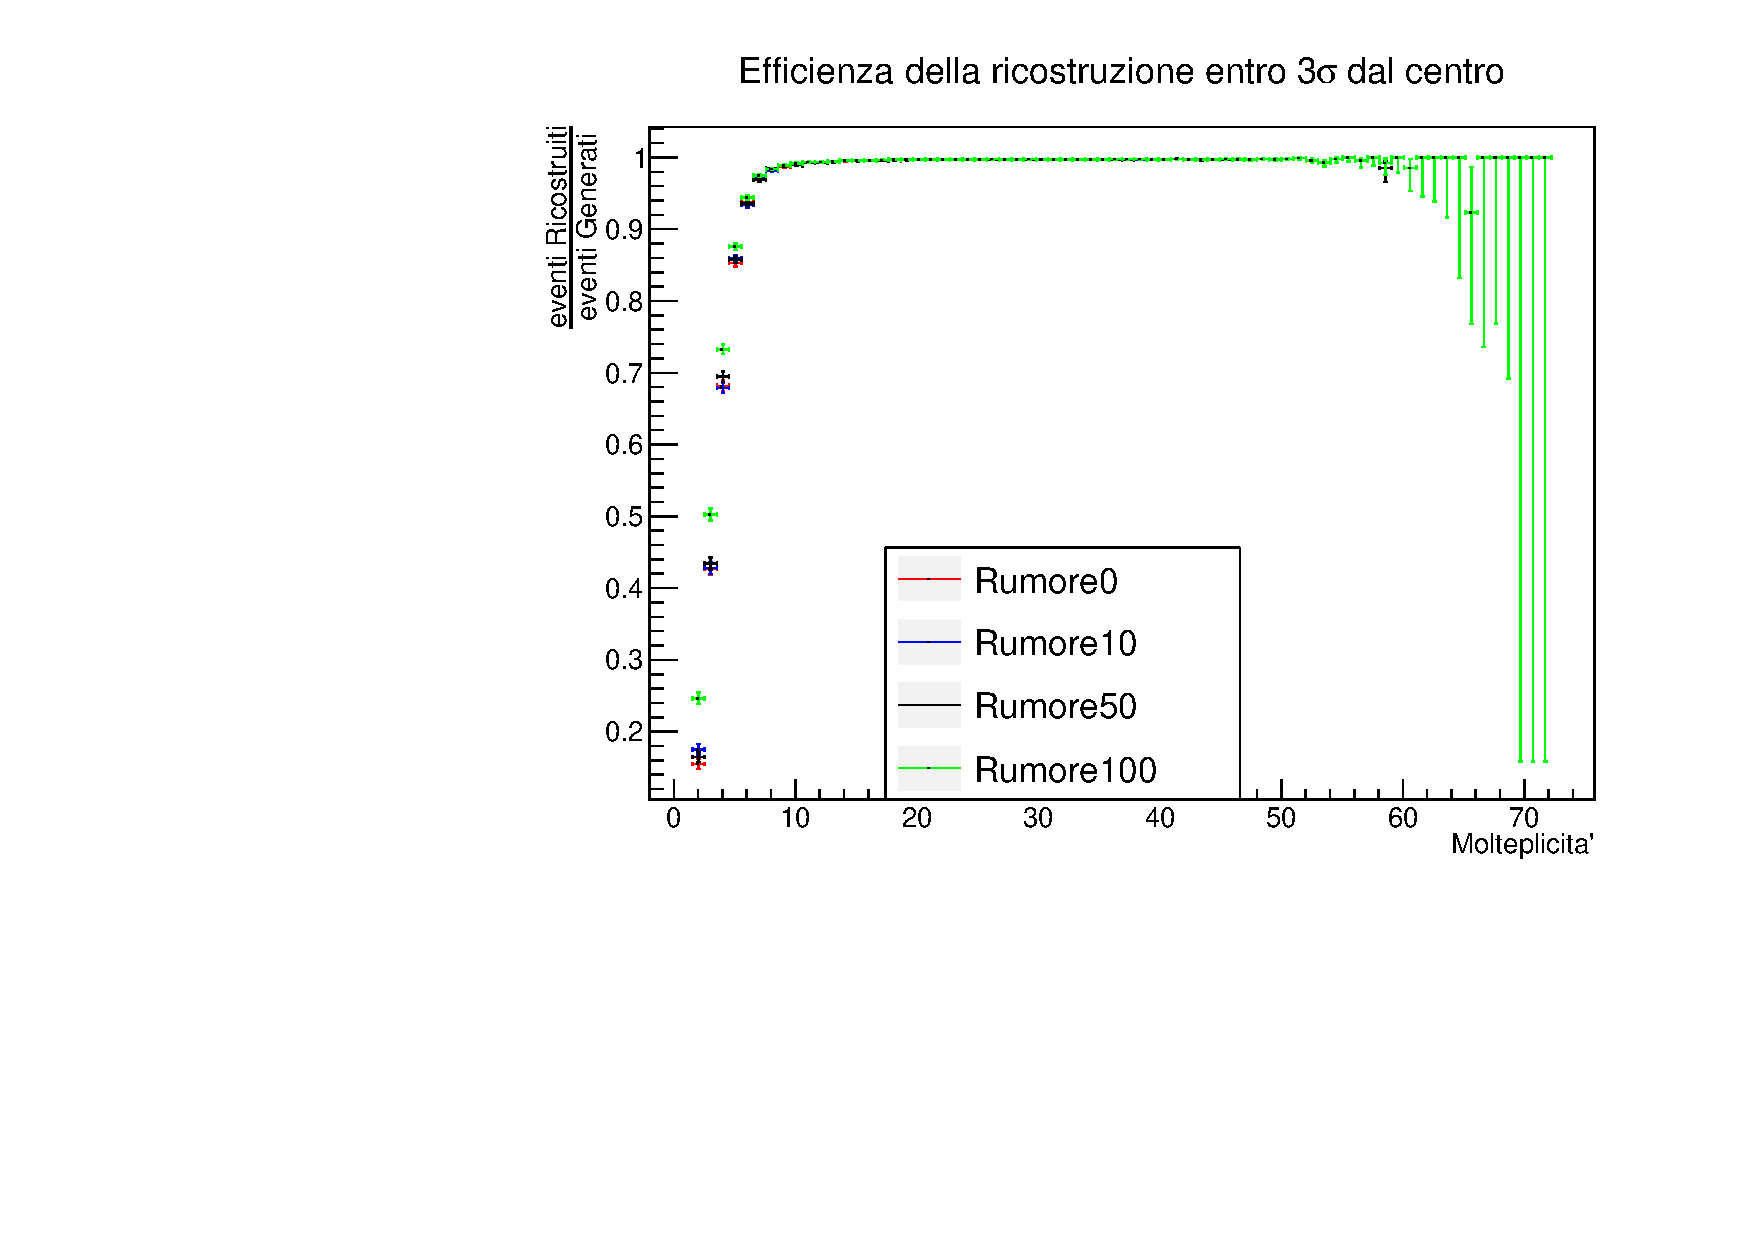
\includegraphics[width=0.95\textwidth]{Immagini/efficienza_molteplicita_2_tutte.pdf}
     %\vspace{-15pt}
     \caption{Efficienza di ricostruzione in funzione della molteplicità valutando gli eventi entro 3$\sigma$}
  \label{effMolt3s}
   \end{minipage}
   \hspace{5mm}
   \begin{minipage}[r]{.47\textwidth}
     \centering
     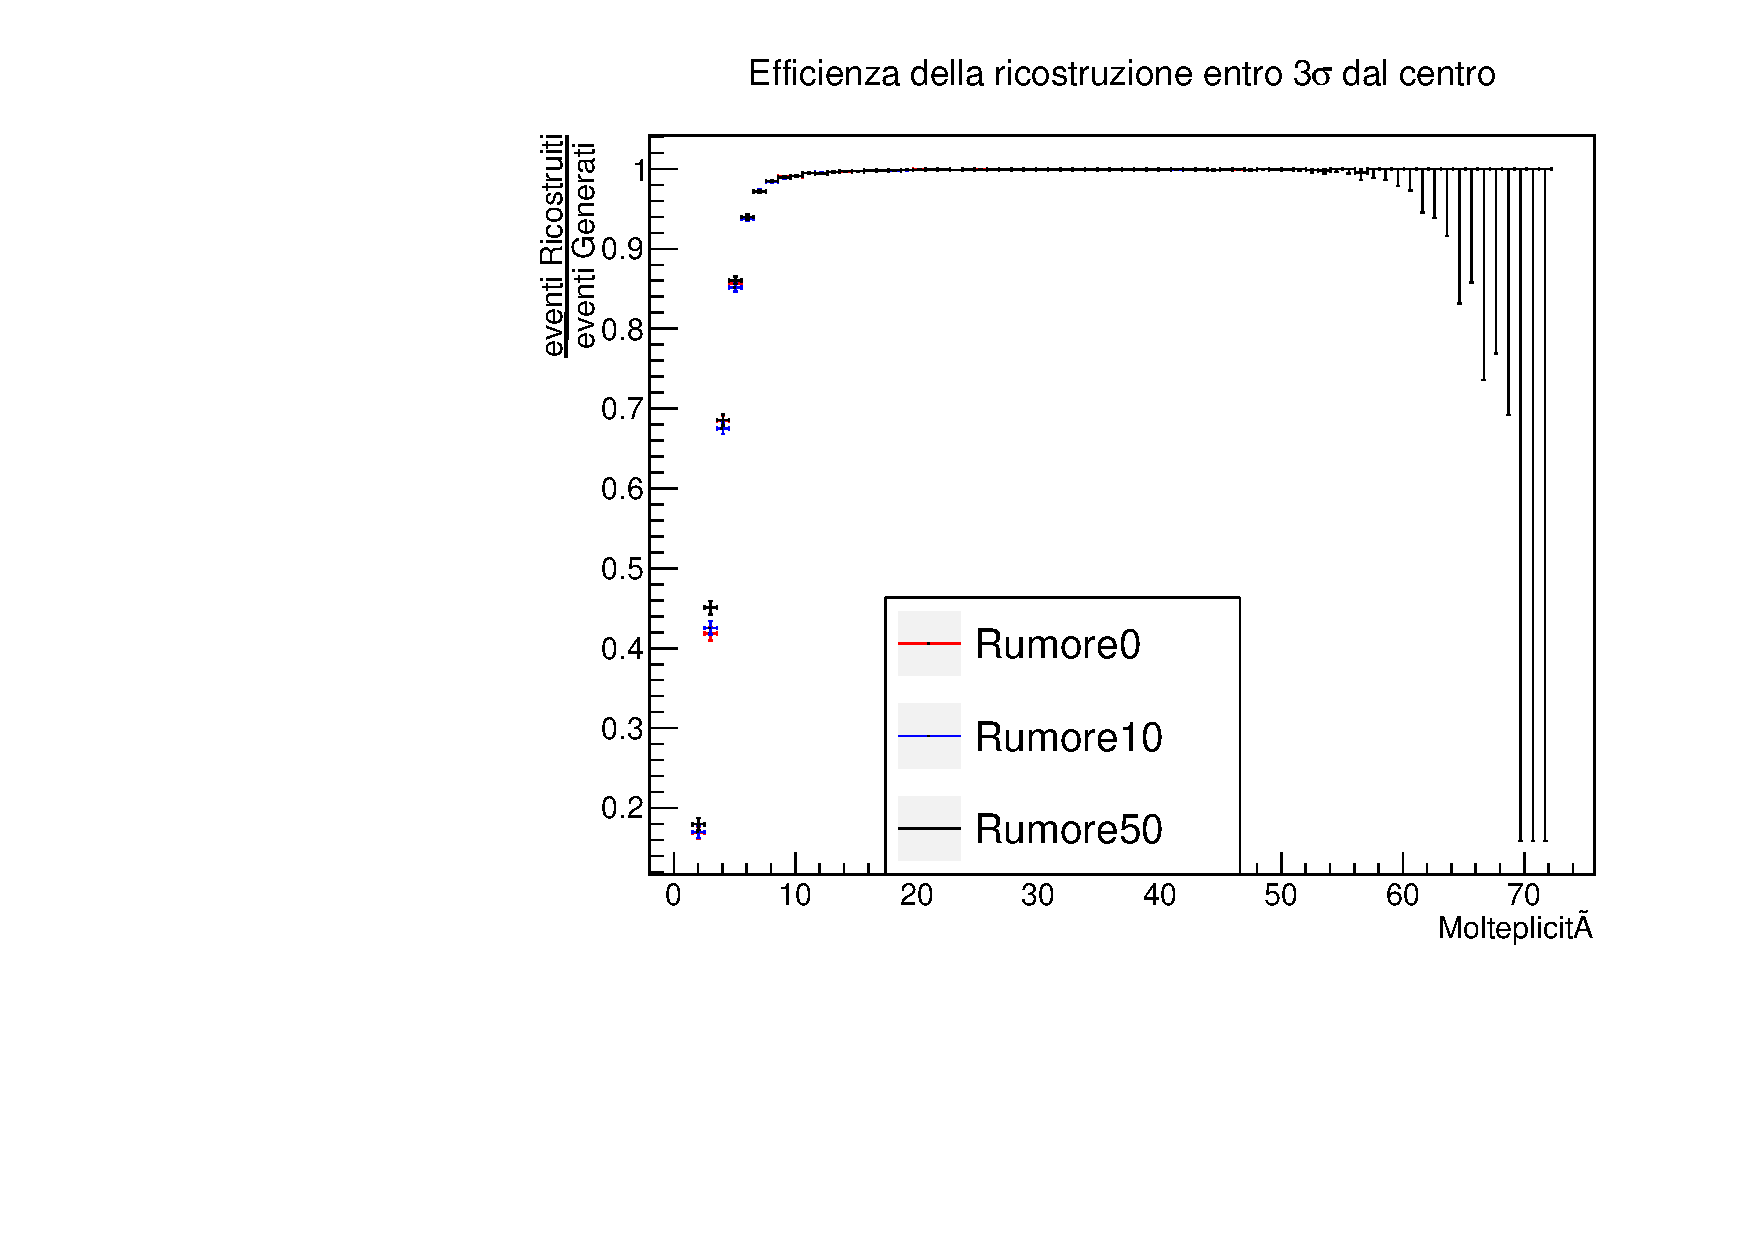
\includegraphics[width=0.95\textwidth]{Immagini/efficienza_molteplicita_2_no_rumore100.pdf}
     %\vspace{-15pt}
     \caption{Efficienza di ricostruzione in funzione della molteplicità valutando gli eventi entro 3$\sigma$ escludendo l'analisi con 100 punti di rumore}
  \label{effMolt3sno100}
   \end{minipage}}
   \vspace{-15pt}
\end{figure}

\end{document}